\documentclass[twoside,11pt]{article}
\usepackage[preprint]{jmlr2e}
\usepackage{amsmath,amssymb,mathtools,bm}
\usepackage{booktabs}
\usepackage{graphicx}
\usepackage{microtype}
\usepackage{url}
\usepackage{xcolor}
\usepackage{algorithm}
\usepackage{algorithmic}
\usepackage{tikz}
\usetikzlibrary{arrows.meta,positioning,calc,fit}

\newcommand{\R}{\mathbb{R}}
\newcommand{\norm}[1]{\left\lVert #1 \right\rVert_2}
\newcommand{\normF}[1]{\left\lVert #1 \right\rVert_F}
\newcommand{\Phir}{\boldsymbol{\Phi}^{\rm ref}}
\newcommand{\Phim}{\boldsymbol{\Phi}^{\rm mdl}}
\newcommand{\Jr}{\mathbf J^{\rm ref}}
\newcommand{\vTG}{\mathbf v_{\rm TG}}
\newcommand{\vadv}{\mathbf v_{\rm adv}}

\jmlrheading{27}{2026}{1--}{--}{--}{--}{Fava}
\ShortHeadings{Realized Error Amplification in Learned Dynamics}{Fava}
\firstpageno{1}

\title{Realized Error Amplification in Learned Dynamical Systems}
\author{\name Thales Coelho Leite Fava \email thalestclf@ita.br\\
       \addr Instituto Tecnol\'ogico de Aeron\'autica\\}
       %Pra\c{c}a Marechal Eduardo Gomes, 50, Vila das Ac\'acias\\
       %12228-900 S\~ao Jos\'e dos Campos, SP, Brazil}

\begin{document}
\maketitle
\begin{abstract}
Learned surrogates with small one-step errors can produce large rollout errors. The current work quantifies how much of the amplification available in the learned dynamics is realized by the defects of the surrogate. To first order, the rollout error is a sum of transported one-step defects, and an exact factorization separates their magnitude, the worst-case propagator gain, the gain efficiency, their cancellation and a nonlinear remainder. For residual multilayer perceptrons trained on Lorenz--96 and Fourier neural operators trained on Kuramoto--Sivashinsky, the worst-case estimate is five to seven times the realized error at about one Lyapunov time. The defects realize the gain expected for random vectors with the same covariance, but their temporal correlation makes the transported defects about four times more coherent than independent ones. The defect magnitude explains the differences between forecasts at short horizons, and the gain and the coherence at longer ones. The disagreement between independently trained surrogates is a reference-free error estimate, which, except for under-trained surrogates, ranks individual forecasts with Spearman correlations of 0.62 to 0.84 up to about one Lyapunov time. Multistep fine-tuning reduces the error of under-trained surrogates by damping their tangent dynamics, but has no consistent effect on converged ones.
\end{abstract}

\begin{keywords}
learned dynamical systems, finite-time amplification, neural operators, error estimation, multistep training
\end{keywords}

\section{Introduction}
\label{sec:intro}

Learned surrogates of dynamical systems are usually trained to predict one step ahead and then used autoregressively, with each prediction fed back as the next input. In this mode of operation, the approximation error made at one step becomes a perturbation of all subsequent states, and a surrogate with a small one-step error can still produce large errors over long rollouts \citep{bengio2015,venkatraman2015,lambert2022}. For this reason, neural weather models and neural PDE solvers are evaluated over many autoregressive steps and are often fine-tuned with multistep objectives \citep{brandstetter2022,lam2023,list2025}.

The growth of a perturbation along a trajectory is governed by the tangent dynamics, and several works use Jacobian information of the learned map to explain or control long-horizon errors, either by regularizing one-step Jacobians \citep{pan2018,nie2026} or by penalizing the non-normality and non-commutativity of consecutive Jacobians, which control the transient amplification available to perturbations \citep{pervez2026}. The leading singular value of a finite-time propagator, however, describes the worst perturbation. The rollout error of a surrogate initialized on the correct state is generated by the defects that the surrogate makes at every step, and whether these defects excite the most amplified directions, and whether their transported contributions reinforce or cancel each other, is not determined by the propagator alone.

The accounting of how local errors are transported and summed is classical in numerical analysis, where the global error of a time integrator is the sum of transported local errors \citep[the ``Lady Windermere's fan'' of][]{hairer1993}, and in predictability studies of model error \citep{nicolis2003,vannitsem2002}. A learned surrogate can be regarded as an inexpensive and imperfect numerical scheme whose local error is the approximation error of the network. Unlike the local error of a classical scheme, this error is not controlled by a truncation order. It is a deterministic and largely unknown function of the state, shaped by the training data and by the architecture, and its interaction with the finite-time geometry of the learned dynamics has to be measured.

The current work quantifies how much of the amplification available in the learned dynamics is realized by the defects of the surrogate. The first-order rollout error is written as a sum of defects transported by reference-trajectory propagators, and an exact factorization splits the rollout error into five factors: the magnitude of the injected defects, the worst-case gain of the tail propagators, the efficiency with which the defects use that gain, the cancellation among the transported defects and the nonlinear remainder. Since the factorization is exact in logarithmic form, the variance of the log-error across initial states is attributed to the five factors without approximation, and the same attribution applies to the difference between two surrogates evaluated on the same forecasts. The conclusion that the realized error depends on the actual defect field, and not on its statistics, is then used to build an error estimate that needs no reference data.

The analysis is applied to residual multilayer perceptrons (MLPs) trained on the 20-dimensional Lorenz--96 system with three optimization budgets, and to Fourier neural operators (FNOs) trained on the Kuramoto--Sivashinsky equation. Horizons are expressed in Lyapunov times, so that the two systems are compared over the same range of chaotic error growth. The main contributions of the current work are the following.
\begin{enumerate}
\item An exact five-factor factorization of the autoregressive rollout error, null models for the efficiency (isotropic and covariance-matched) and for the vector composition (coherent, incoherent and bias-only limits), and an exact variance attribution of the log-error (Section~\ref{sec:accounting}).
\item Evidence, for two systems, two architectures and a sixtyfold range of one-step accuracy, that the defects realize, within 7\%, the fraction of the worst-case gain expected for random vectors with their own covariance. The decrease of the efficiency with the horizon follows from the singular spectrum of the propagators (Section~\ref{sec:res_efficiency}).
\item Evidence that the transported defects are strongly coherent, about four times more than independent defects, and that the coherence comes from the temporal correlation of the defects along the trajectory and not from a systematic bias (Section~\ref{sec:res_coherence}).
\item A variance attribution showing that the defect magnitude explains the differences between forecasts at short horizons, and that the worst-case gain, the coherence and, for the FNOs, the orientation of the defects take over beyond about half a Lyapunov time, with a similar budget for all accuracy levels (Section~\ref{sec:res_budget}).
\item A reference-free error estimate in which the disagreement between independently trained surrogates replaces the unknown defects. Except for the under-trained Lorenz--96 surrogates, it ranks individual forecasts up to about one Lyapunov time and is calibrated in magnitude for the converged ones, whereas scores built from the defect statistics do not rank the forecasts (Section~\ref{sec:res_ensemble}).
\item A diagnosis of multistep fine-tuning. It reduces the error of under-trained surrogates, whose free rollouts leave the attractor, by lowering the gain of their tangent dynamics, and it has no consistent effect on surrogates that reproduce the reference tangent dynamics (Sections~\ref{sec:res_fidelity} and \ref{sec:res_intervention}).
\end{enumerate}

\begin{figure}[t]
\centering
\resizebox{\textwidth}{!}{%
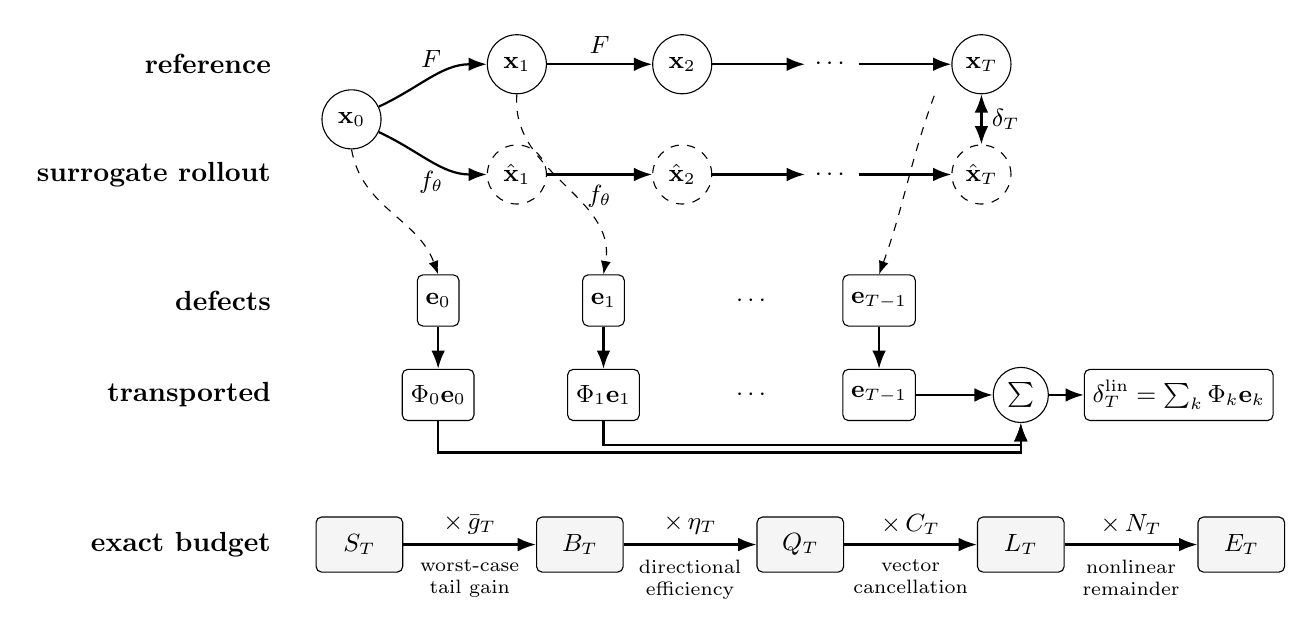
\begin{tikzpicture}[
    >=Latex, font=\small,
    st/.style={circle, draw, minimum size=7.5mm, inner sep=1pt},
    box/.style={rectangle, draw, rounded corners=2pt, minimum height=6.5mm, inner sep=3pt, align=center},
    fbox/.style={rectangle, draw, rounded corners=2pt, minimum height=7mm, minimum width=11mm, inner sep=3pt, align=center, fill=black!4},
    flow/.style={->, thick},
    defect/.style={->, dashed},
]
% trajectories ------------------------------------------------------------
\node[font=\bfseries, anchor=east] at (-0.4,2.4) {reference};
\node[font=\bfseries, anchor=east] at (-0.4,1.0) {surrogate rollout};
\node[st] (x0) at (0.5,1.7) {$\mathbf x_0$};
\node[st] (x1) at (2.6,2.4) {$\mathbf x_1$};
\node[st] (x2) at (4.7,2.4) {$\mathbf x_2$};
\node (d1) at (6.6,2.4) {$\cdots$};
\node[st] (xT) at (8.5,2.4) {$\mathbf x_T$};
\draw[flow] (x0) to[out=25,in=180] node[above] {$F$} (x1);
\draw[flow] (x1) -- node[above] {$F$} (x2);
\draw[flow] (x2) -- (d1); \draw[flow] (d1) -- (xT);
\node[st,dashed] (h1) at (2.6,1.0) {$\hat{\mathbf x}_1$};
\node[st,dashed] (h2) at (4.7,1.0) {$\hat{\mathbf x}_2$};
\node (d2) at (6.6,1.0) {$\cdots$};
\node[st,dashed] (hT) at (8.5,1.0) {$\hat{\mathbf x}_T$};
\draw[flow] (x0) to[out=-25,in=180] node[below] {$f_\theta$} (h1);
\draw[flow] (h1) -- node[below] {$f_\theta$} (h2);
\draw[flow] (h2) -- (d2); \draw[flow] (d2) -- (hT);
\draw[<->, thick] (xT) -- node[right] {$\delta_T$} (hT);
% defects and transport ------------------------------------------------------
\node[font=\bfseries, anchor=east] at (-0.4,-0.6) {defects};
\node[font=\bfseries, anchor=east] at (-0.4,-1.8) {transported};
\node[box] (e0) at (1.6,-0.6) {$\mathbf e_0$};
\node[box] (e1) at (3.7,-0.6) {$\mathbf e_1$};
\node at (5.6,-0.6) {$\cdots$};
\node[box] (ek) at (7.2,-0.6) {$\mathbf e_{T-1}$};
\node[box] (q0) at (1.6,-1.8) {$\Phi_0\mathbf e_0$};
\node[box] (q1) at (3.7,-1.8) {$\Phi_1\mathbf e_1$};
\node at (5.6,-1.8) {$\cdots$};
\node[box] (qk) at (7.2,-1.8) {$\mathbf e_{T-1}$};
\draw[defect] (x0.south) to[out=-80,in=110] (e0.north);
\draw[defect] (x1.south) to[out=-95,in=80] (e1.north);
\draw[defect] (7.9,2.0) to[out=-110,in=70] (ek.north);
\draw[flow] (e0) -- (q0); \draw[flow] (e1) -- (q1); \draw[flow] (ek) -- (qk);
\node[circle, draw, minimum size=7mm, inner sep=0pt] (sum) at (9.0,-1.8) {$\sum$};
\draw[flow] (q0.south) -- ++(0,-0.4) -| (sum.south);
\draw[flow] (q1.south) -- ++(0,-0.3) -| (sum.south);
\draw[flow] (qk.east) -- (sum.west);
\node[box, anchor=west] (lin) at (9.8,-1.8) {$\delta^{\rm lin}_T=\sum_k\Phi_k\mathbf e_k$};
\draw[flow] (sum) -- (lin);
% factor chain ---------------------------------------------------------------
\node[font=\bfseries, anchor=east] at (-0.4,-3.7) {exact budget};
\node[fbox] (f1) at (0.6,-3.7) {$S_T$};
\node[fbox] (f2) at (3.4,-3.7) {$B_T$};
\node[fbox] (f3) at (6.2,-3.7) {$Q_T$};
\node[fbox] (f4) at (9.0,-3.7) {$L_T$};
\node[fbox] (f5) at (11.8,-3.7) {$E_T$};
\draw[flow] (f1) -- node[above] {$\times\,\bar g_T$} node[below=0.6mm, font=\scriptsize, align=center] {worst-case\\tail gain} (f2);
\draw[flow] (f2) -- node[above] {$\times\,\eta_T$} node[below=0.6mm, font=\scriptsize, align=center] {directional\\efficiency} (f3);
\draw[flow] (f3) -- node[above] {$\times\,C_T$} node[below=0.6mm, font=\scriptsize, align=center] {vector\\cancellation} (f4);
\draw[flow] (f4) -- node[above] {$\times\,N_T$} node[below=0.6mm, font=\scriptsize, align=center] {nonlinear\\remainder} (f5);
\end{tikzpicture}%
}
\caption{Realized error amplification. The reference map $F$ and the surrogate $f_\theta$ start from the same state. At every reference state the surrogate injects a defect $\mathbf e_k=f_\theta(\mathbf x_k)-\mathbf x_{k+1}$, which the tail propagator $\Phi_k=\Phir(T,k+1)$ transports to the forecast time ($\Phi_{T-1}=I$), and the transported defects are summed. The rollout error factorizes exactly into the injected magnitude $S_T=\sum_k\|\mathbf e_k\|_2$ and four factors: the worst-case gain of the tail propagators ($B_T=\sum_k\sigma_1(\Phi_k)\|\mathbf e_k\|_2$), the fraction of that gain realized by the defect directions ($Q_T=\sum_k\|\Phi_k\mathbf e_k\|_2$), the cancellation in the vector sum ($L_T=\|\delta^{\rm lin}_T\|_2$) and the nonlinear remainder ($E_T=\|\delta_T\|_2$); see Proposition~\ref{prop:factorization}.}
\label{fig:concept}
\end{figure}

\section{Related Work}
\label{sec:related}

\paragraph{Global error of numerical schemes and model error in forecasting.}
The representation of a global error as a sum of transported local errors is classical in the numerical analysis of time integrators \citep[Section~II.3]{hairer1993}, where it also underlies a posteriori error estimation by adjoint (dual) problems \citep{estep1995,cao2004,giles2002}. In predictability studies, the same forced linear equation describes the growth of model error \citep{orrell2001}: \citet{nicolis2003,nicolis2004} derived the short-time evolution of the mean-square error caused by model imperfections, and \citet{vannitsem2002} showed that this evolution is linear or quadratic in time depending on the temporal correlation of the error source, the quadratic case being the generic one. The current work brings this point of view to learned surrogates, whose local errors are neither a truncation error of known order nor a prescribed stochastic process, and adds an exact decomposition of the realized error together with null models that separate the generic effect of the propagator from the structure of the defects.

\paragraph{Non-modal amplification, stochastic forcing and Lyapunov vectors.}
Non-normal linear operators can amplify perturbations transiently even when they are asymptotically stable \citep{trefethen1993,reddy1993,schmid2007}, and the optimal initial perturbation is given by the leading right singular vector of the finite-time propagator. For forced systems, generalized stability theory replaces the optimal perturbation by the response to stochastic forcing with a prescribed covariance, described by finite-time Gramians \citep{farrell1996a,farrell1996b}, and input--output analyses of fluid flows quantify the amplification from forcing to response \citep{jovanovic2005}. At long times, singular vectors of the propagator converge to Lyapunov vectors \citep{legras1996,ginelli2007,kuptsov2012}. Non-normal transient responses have also been studied in recurrent neural circuits \citep{hennequin2012} and in the optimization dynamics of neural networks \citep{ghosh2026}. Here the parameters of the surrogate are fixed, and these tools are used to characterize how the defects of a trained model populate the singular spectrum of its tangent dynamics.

\paragraph{Compounding error and long-horizon training of learned dynamics.}
The mismatch between training on reference inputs and testing on the model's own outputs is well known in sequence prediction \citep{bengio2015,venkatraman2015} and in model-based control \citep{lambert2022}. For chaotic systems, recurrent models face exploding gradients whose rate is set by the Lyapunov spectrum, which motivates teacher forcing and its generalizations \citep{mikhaeil2022,hess2023}, and statistical accuracy of learned chaotic dynamics has been related to the accuracy of their Jacobians and to shadowing \citep{park2024}. Long rollouts of neural PDE solvers and weather models are improved by multistep or unrolled objectives \citep{brandstetter2022,list2025,lam2023}, by architectural choices that control spectral content or instability \citep{lippe2023,mccabe2023}, and by inference-time corrections \citep{pedersen2025}. Jacobian regularization has been proposed to improve long-time prediction \citep{pan2018,nie2026}, and \citet{pervez2026} penalize the non-normality and non-commutativity of consecutive Jacobians, which control the transient amplification available along a rollout. These works act on the available amplification or on the training objective. The current work is diagnostic: it measures how much of the available amplification is realized by the defects of a fixed surrogate and which factor makes some forecasts worse than others, and it applies the same accounting to the effect of a multistep objective.

\paragraph{Ensembles and error estimates without reference data.}
Ensemble forecasting estimates the uncertainty of a numerical weather prediction from the spread of perturbed forecasts \citep{leutbecher2008}, and deep ensembles estimate the predictive uncertainty of neural networks from the disagreement between independently trained members \citep{lakshminarayanan2017}. A posteriori error estimates of numerical schemes, on the other hand, transport computable local residuals with the tangent or adjoint dynamics \citep{estep1995,cao2004,giles2002}. The reference-free test of the current work combines the two ideas: the disagreement between independently trained surrogates estimates the local defect, and the forced recursion transports it along the forecast.

\paragraph{Benchmarks.}
Lorenz--96 \citep{lorenz1996} and the Kuramoto--Sivashinsky equation are standard testbeds for data-driven forecasting of chaotic dynamics \citep{vlachas2018,pathak2018}. Fourier neural operators parameterize global convolutions in Fourier space \citep{li2021} and provide a surrogate class that differs from the finite-dimensional residual MLP in both representation and inductive bias.

\section{Forced Error Recursion and Finite-Time Propagators}
\label{sec:formulation}

Let the reference dynamics and the learned one-step surrogate be the discrete maps
\begin{align}
  \mathbf x_{k+1} &= F(\mathbf x_k), \label{eq:true_map}\\
  \hat{\mathbf x}_{k+1} &= f_\theta(\hat{\mathbf x}_k), \label{eq:learned_map}
\end{align}
with $\mathbf x_k,\hat{\mathbf x}_k\in\R^d$. The accumulated rollout error and the local defect are
\begin{equation}
  \delta_k=\hat{\mathbf x}_k-\mathbf x_k,
  \qquad
  \mathbf e_k=f_\theta(\mathbf x_k)-F(\mathbf x_k)=f_\theta(\mathbf x_k)-\mathbf x_{k+1}.
  \label{eq:delta_defect}
\end{equation}
The defect $\mathbf e_k$ is the error made by the surrogate in a single step when it is fed the correct state, whereas $\delta_k$ is the error accumulated after the surrogate has been fed its own outputs.

\subsection{Reference-trajectory linearization}

Let $\Jr_k=Df_\theta(\mathbf x_k)$ be the Jacobian of the surrogate at the reference state. A Taylor expansion of $f_\theta(\mathbf x_k+\delta_k)$ about $\mathbf x_k$ gives the forced error recursion
\begin{equation}
  \delta_{k+1}=\Jr_k\delta_k+\mathbf e_k+\mathbf r_k,
  \qquad
  \mathbf r_k=f_\theta(\mathbf x_k+\delta_k)-f_\theta(\mathbf x_k)-\Jr_k\delta_k,
  \label{eq:error_recursion}
\end{equation}
where $\mathbf r_k$ contains the second- and higher-order terms. For $s_2>s_1$, the ordered reference-trajectory propagator is
\begin{equation}
  \Phir(s_2,s_1)=\Jr_{s_2-1}\Jr_{s_2-2}\cdots\Jr_{s_1},
  \qquad \Phir(s,s)=I.
  \label{eq:reference_propagator}
\end{equation}
Without loss of generality, the forecast window starts at $k=0$ and ends at $k=T$. Repeated substitution of Eq.~\eqref{eq:error_recursion} gives the exact identity (Appendix~\ref{app:derivation})
\begin{equation}
\delta_{T}=\Phir(T,0)\,\delta_0+\sum_{k=0}^{T-1}\Phi_k\left(\mathbf e_{k}+\mathbf r_{k}\right),
\qquad
\Phi_k:=\Phir(T,k+1),
\label{eq:error_decomposition}
\end{equation}
where $\Phi_k$ is the tail propagator that transports a defect injected at step $k$ to the forecast time. A rollout initialized on the reference state has $\delta_0=0$, so that, neglecting the remainders,
\begin{equation}
  \boxed{\;
  \delta^{\rm lin}_{T}=\sum_{k=0}^{T-1}\mathbf q_k,
  \qquad
  \mathbf q_k=\Phi_k\mathbf e_k.
  \;}
  \label{eq:linear_error_prediction}
\end{equation}
In Eq.~\eqref{eq:linear_error_prediction}, the defects act as forcing terms, the tail propagators transport them to a common time, and the transported vectors are summed. The difference $\delta_T-\delta^{\rm lin}_T=\sum_k\Phi_k\mathbf r_k$ is computed explicitly in the experiments, so that the validity of the first-order description is measured rather than assumed. A local bound on $\mathbf r_k$ is given in Appendix~\ref{app:remainder}.

Equation~\eqref{eq:linear_error_prediction} is the global-error formula of numerical analysis \citep[Section~II.3]{hairer1993} and the discrete form of the model-error equation of predictability studies \citep{nicolis2003,vannitsem2002,carrassi2008}, with the approximation error of the network in place of a truncation error or a prescribed random process.

\subsection{Model-trajectory propagator}

A second propagator describes perturbations of the learned rollout itself. With $\bar{\mathbf x}_0=\mathbf x_0$ and $\bar{\mathbf x}_{j+1}=f_\theta(\bar{\mathbf x}_j)$,
\begin{equation}
  \Phim(T,0)=Df_\theta(\bar{\mathbf x}_{T-1})\cdots Df_\theta(\bar{\mathbf x}_0)=Df_\theta^{(T)}(\mathbf x_0).
  \label{eq:model_propagator}
\end{equation}
The reference propagator $\Phir$ appears in the expansion of the ordinary rollout error about the reference trajectory, whereas $\Phim$ is the derivative of the autonomous rollout and is the appropriate object for perturbations of the initial condition or for adversarial stress tests. The two coincide only while the rollout remains close to the reference, and $\Phim$ is used in Section~\ref{sec:design_ensemble} and Appendix~\ref{app:stress}.

\section{An Exact Account of the Realized Error}
\label{sec:accounting}

The worst-case finite-time gain of the reference propagator,
\begin{equation}
  G_{\max}(T)=\sigma_1^2\!\left[\Phir(T,0)\right],
  \label{eq:gmax}
\end{equation}
measures the largest amplification available to an infinitesimal perturbation of the initial state. Its maximizing direction is the leading right singular vector of $\Phir(T,0)$, which is the optimal perturbation of transient-growth analysis \citep{reddy1993,schmid2007}. For a forced problem, the analogous worst case is the gain of the forcing-to-error map $\mathcal L_T=[\Phi_0,\Phi_1,\ldots,\Phi_{T-1}]\in\R^{d\times dT}$,
\begin{equation}
  \|\delta^{\rm lin}_T\|_2\le\|\mathcal L_T\|_2\Big(\sum_k\|\mathbf e_k\|_2^2\Big)^{1/2},
  \qquad
  \|\mathcal L_T\|_2^2=\lambda_{\max}\Big(\sum_k\Phi_k\Phi_k^\top\Big),
  \label{eq:forced_gain}
\end{equation}
whose square is the largest eigenvalue of the finite-time controllability Gramian, the quantity that generalized stability theory associates with optimal forcing \citep{farrell1996b}. Both quantities describe what the learned dynamics could do to some perturbation or forcing. The rollout error, on the other hand, is produced by one particular sequence of defects. This section decomposes the rollout error into the magnitude of that sequence and a few dimensionless factors that measure how much of the available amplification it realizes.

\subsection{Five-factor factorization}

Let $\sigma_1(\Phi_k)$ be the leading singular value of the tail propagator and define the totals
\begin{equation}
  S_T=\sum_{k=0}^{T-1}\|\mathbf e_k\|_2,
  \qquad
  B_T=\sum_{k=0}^{T-1}\sigma_1(\Phi_k)\,\|\mathbf e_k\|_2,
  \qquad
  Q_T=\sum_{k=0}^{T-1}\|\mathbf q_k\|_2,
  \label{eq:totals}
\end{equation}
together with $L_T=\|\delta^{\rm lin}_T\|_2$ and the rollout error $E_T=\|\delta_T\|_2$. By the triangle inequality and the definition of the spectral norm, $L_T\le Q_T\le B_T$, so that $B_T$ is the first-order worst-case bound on the error produced by the actual defect magnitudes.

\begin{proposition}[Exact factorization]
\label{prop:factorization}
If the defects and the first-order error are nonzero,
\begin{equation}
  \boxed{\;E_T=S_T\cdot\bar g_T\cdot\eta_T\cdot C_T\cdot N_T,\;}
  \label{eq:factorization}
\end{equation}
with
\begin{equation}
  \bar g_T=\frac{B_T}{S_T}=\sum_k w_k\,\sigma_1(\Phi_k),
  \qquad
  \eta_T=\frac{Q_T}{B_T}=\sum_k v_k\,\eta_k,
  \qquad
  C_T=\frac{L_T}{Q_T},
  \qquad
  N_T=\frac{E_T}{L_T},
  \label{eq:factors}
\end{equation}
where $w_k=\|\mathbf e_k\|_2/S_T$ and $v_k=\sigma_1(\Phi_k)\|\mathbf e_k\|_2/B_T$ are weights summing to one, and
\begin{equation}
  \eta_k=\frac{\|\Phi_k\mathbf e_k\|_2}{\sigma_1(\Phi_k)\,\|\mathbf e_k\|_2}\in[a_k,1],
  \qquad
  a_k=\frac{|\mathbf v_{k1}^\top\mathbf e_k|}{\|\mathbf e_k\|_2},
  \label{eq:gain_efficiency}
\end{equation}
is the efficiency of the defect injected at step $k$, $a_k$ its alignment with the leading right singular vector $\mathbf v_{k1}$ of $\Phi_k$. Moreover $\eta_T\in(0,1]$ and $C_T\in[0,1]$.
\end{proposition}

The product telescopes, and the bounds follow from $\|\Phi_k\mathbf e_k\|_2^2=\sum_i\sigma_{ki}^2(\mathbf v_{ki}^\top\mathbf e_k)^2\ge\sigma_{k1}^2a_k^2\|\mathbf e_k\|_2^2$ and from the triangle inequality (Appendix~\ref{app:proofs}). The five factors have a direct interpretation. $S_T$ is the total defect injected along the window, $\bar g_T$ is the worst-case tail gain seen by a typical unit of defect, $\eta_T$ measures how much of that gain the actual defect directions realize, $C_T$ measures how much of the transported magnitude survives the vector sum, and $N_T=R_{\rm lin}^{-1}$, with $R_{\rm lin}=L_T/E_T$, measures the departure from the first-order description. The product $S_T\bar g_T=B_T$ is a worst-case estimate, and the remaining factors are the attenuations that turn it into the realized error.

\subsection{Null models for the efficiency}

Small values of $\eta_T$ do not by themselves indicate that the defects avoid the amplified directions, since a generic vector projects weakly on a single direction in high dimension. The efficiency is therefore compared with the value expected for random defects.

\begin{proposition}[Isotropic and covariance-matched efficiencies]
\label{prop:nulls}
Let $\Phi\in\R^{d\times d}$ have singular values $\sigma_1\ge\cdots\ge\sigma_d$ and right singular vectors $\mathbf v_i$.
\begin{enumerate}
\item If $\mathbf u$ is uniformly distributed on the unit sphere, $\mathbb E\|\Phi\mathbf u\|_2^2=\|\Phi\|_F^2/d$, and the root-mean-square efficiency of a random direction is
\begin{equation}
  \eta^{\rm iso}(\Phi)=\frac{(\mathbb E\|\Phi\mathbf u\|_2^2)^{1/2}}{\sigma_1}=\left(\frac{r(\Phi)}{d}\right)^{1/2},
  \qquad
  r(\Phi)=\frac{\|\Phi\|_F^2}{\sigma_1^2}\in[1,d],
  \label{eq:eta_iso}
\end{equation}
where $r(\Phi)$ is the stable rank.
\item If $\mathbf e$ is a random vector with second moment $\Sigma=\mathbb E[\mathbf e\mathbf e^\top]$, then $\mathbb E\|\Phi\mathbf e\|_2^2=\operatorname{tr}(\Phi\Sigma\Phi^\top)=\sum_i\sigma_i^2\,\mathbf v_i^\top\Sigma\mathbf v_i$, and the covariance-matched efficiency is
\begin{equation}
  \eta^{\Sigma}(\Phi)=\frac{g_\Sigma(\Phi)}{\sigma_1},
  \qquad
  g_\Sigma(\Phi)=\left(\frac{\operatorname{tr}(\Phi\Sigma\Phi^\top)}{\operatorname{tr}\Sigma}\right)^{1/2}.
  \label{eq:eta_cov}
\end{equation}
\item If $\sigma_2/\sigma_1\to0$, then $\eta^{\rm iso}\to d^{-1/2}$ and $\eta^{\Sigma}\to(\mathbf v_1^\top\Sigma\mathbf v_1/\operatorname{tr}\Sigma)^{1/2}$.
\end{enumerate}
\end{proposition}

The proof is given in Appendix~\ref{app:proofs}. The gain $g_\Sigma$ is the variance amplification of a perturbation with covariance $\Sigma$, the quantity used by generalized stability theory for stochastically forced dynamics \citep{farrell1996a,farrell1996b}. In the third statement, $\mathbf v_1$ is the leading right singular vector of a long tail propagator, which approaches the leading forward Lyapunov vector at the injection time \citep{legras1996,kuptsov2012}, so that, at long horizons, the efficiency of random defects measures the fraction of the defect variance carried along that vector.

The closed forms of Proposition~\ref{prop:nulls} are root-mean-square gains, whereas $\eta_k$ is a ratio of norms. By Jensen's inequality, $\mathbb E[\|\Phi\mathbf u\|_2/\|\mathbf u\|_2]\le(\mathbb E[\|\Phi\mathbf u\|_2^2/\|\mathbf u\|_2^2])^{1/2}$, and the gap is not small. For a rank-one propagator and Gaussian $\mathbf u$ in high dimension, the ratio between the two approaches $(2/\pi)^{1/2}\approx0.80$, which is the typical regime of long tails, so that the efficiency is compared with the mean norm gain
\begin{equation}
  \bar g_\Sigma(\Phi)=\mathbb E\left[\frac{\|\Phi\mathbf u\|_2}{\|\mathbf u\|_2}\right],
  \qquad \mathbf u\sim\mathcal N(\mathbf 0,\Sigma),
  \label{eq:mean_gain}
\end{equation}
which is estimated with 64 Monte Carlo draws per tail propagator (the same draws for all propagators of a window), and the window-level null and orientation ratio are
\begin{equation}
  \eta^{\Sigma}_T=\frac{1}{B_T}\sum_k \bar g_\Sigma(\Phi_k)\,\|\mathbf e_k\|_2,
  \qquad
  \alpha_T=\frac{\eta_T}{\eta^{\Sigma}_T}=\frac{Q_T}{\sum_k\bar g_\Sigma(\Phi_k)\,\|\mathbf e_k\|_2}.
  \label{eq:alpha}
\end{equation}
The isotropic null $\eta^{\rm iso}_T$ uses $\Sigma=I$. The orientation ratio $\alpha_T$ is close to one when the defects of a window are oriented like random vectors with the same second moment and magnitudes, and exceeds one when they are better aligned with the amplified directions. In the experiments, $\Sigma$ is estimated from the defects of the surrogate on an independent trajectory, so that $\eta^\Sigma_T$ uses only information available before the forecast.

\subsection{Cancellation, coherence and the number of contributions}

The cancellation ratio $C_T$ depends on how many contributions of comparable size enter the sum and on how they are oriented with respect to each other. These two effects are separated by writing
\begin{equation}
  C_T=\frac{\kappa_T}{T_{\rm eff}^{1/2}},
  \qquad
  T_{\rm eff}=\frac{Q_T^2}{\sum_k\|\mathbf q_k\|_2^2}\in[1,T],
  \qquad
  \kappa_T=\frac{L_T}{\left(\sum_k\|\mathbf q_k\|_2^2\right)^{1/2}},
  \label{eq:coherence}
\end{equation}
where $T_{\rm eff}$ is the effective number of injection times that contribute to the error and $\kappa_T$ is a coherence factor.

\begin{proposition}[Coherent and incoherent composition]
\label{prop:coherence}
(i) $0\le\kappa_T\le T_{\rm eff}^{1/2}$, with $\kappa_T=T_{\rm eff}^{1/2}$ if and only if all nonzero $\mathbf q_k$ are positively collinear. (ii) If the $\mathbf q_k$ are random with $\mathbb E[\mathbf q_j^\top\mathbf q_k]=0$ for $j\ne k$, then $\mathbb E L_T^2=\sum_k\mathbb E\|\mathbf q_k\|_2^2$, and $\kappa_T=1$ is the incoherent reference. (iii) If $\Phi_k\approx I$ and $\|\mathbf e_k\|_2=\epsilon$ for all $k$, a persistent defect gives $L_T\approx T\epsilon$, whereas mutually uncorrelated defects give $L_T\approx T^{1/2}\epsilon$.
\end{proposition}

The third statement recovers the two short-time regimes of model-error growth discussed by \citet{vannitsem2002}, in which the mean-square error grows quadratically for a persistent or slowly varying error source and linearly for a white one. The coherence factor generalizes this distinction to arbitrary horizons, with $\kappa_T=T_{\rm eff}^{1/2}$ for perfectly coherent transported defects and $\kappa_T\approx1$ for incoherent ones.

A coherent sum can have two different causes. The defects may share a nonzero mean, that is, a systematic bias of the surrogate, or they may be correlated in time because consecutive states of the trajectory are close and the defect is a smooth function of the state. The two causes are separated by the coherence expected for defects drawn independently at every step from a distribution with the mean $\boldsymbol\mu$ and the second moment $\Sigma$ of the actual defects. For such defects,
\begin{equation}
  \mathbb E\,L_T^2=\sum_k\operatorname{tr}\!\left(\Phi_k(\Sigma-\boldsymbol\mu\boldsymbol\mu^\top)\Phi_k^\top\right)+\Big\|\sum_k\Phi_k\boldsymbol\mu\Big\|_2^2,
  \qquad
  \mathbb E\sum_k\|\mathbf q_k\|_2^2=\sum_k\operatorname{tr}\!\left(\Phi_k\Sigma\Phi_k^\top\right),
  \label{eq:kappa_iid}
\end{equation}
and the bias-only coherence is $\kappa^{\rm iid}_T=(\mathbb E L_T^2/\mathbb E\sum_k\|\mathbf q_k\|_2^2)^{1/2}$. It equals one for unbiased defects and grows with the transported bias $\sum_k\Phi_k\boldsymbol\mu$. The ratio $\kappa_T/\kappa^{\rm iid}_T$ measures the coherence produced by the temporal correlation of the defects along the trajectory. Equation~\eqref{eq:kappa_iid} follows from $\mathbb E[\mathbf q_j^\top\mathbf q_k]=\boldsymbol\mu^\top\Phi_j^\top\Phi_k\boldsymbol\mu$ for $j\neq k$.

\subsection{Occupation of the singular spectrum}

For a tail propagator with singular value decomposition $\Phi_k=U_k\Sigma_kV_k^\top$ and coefficients $c_{ki}=\mathbf v_{ki}^\top\mathbf e_k$, the transported energy decomposes exactly as $\|\Phi_k\mathbf e_k\|_2^2=\sum_i\sigma_{ki}^2c_{ki}^2$. The fractions
\begin{equation}
  \begin{gathered}
  p_{ki}=\frac{\sigma_{ki}^2c_{ki}^2}{\sum_j\sigma_{kj}^2c_{kj}^2},
  \qquad
  P_{k,m}=\sum_{i=1}^{m}p_{ki},
  \\
  m_{90,k}=\min\{m:P_{k,m}\ge0.9\},
  \qquad
  N_{{\rm part},k}=\Big(\sum_ip_{ki}^2\Big)^{-1},
  \end{gathered}
  \label{eq:spectral}
\end{equation}
describe how many singular directions carry the transported energy of a defect. Fractions inside exactly degenerate singular subspaces depend on the basis and are interpreted at the subspace level only. For an isotropic random defect, $\mathbb E[c_{ki}^2]$ does not depend on $i$, so that $p_{ki}$ is, on average, proportional to $\sigma_{ki}^2$. Any concentration of the transported energy that follows the spreading of the singular values is therefore expected for arbitrary defects. Statistics of actual defects are compared with Monte Carlo draws of isotropic and covariance-matched random defects under the same tail propagators.

\subsection{Attribution of error variability}

Since Eq.~\eqref{eq:factorization} is a product, its logarithm is a sum, and the variability of the log-error across forecast windows can be attributed to the factors exactly.

\begin{proposition}[Covariance attribution]
\label{prop:attribution}
For any collection of windows with $\log E_T=\sum_j\log X_j$,
\begin{equation}
  \operatorname{Var}(\log E_T)=\sum_j\operatorname{Cov}(\log E_T,\log X_j),
  \qquad
  s_j=\frac{\operatorname{Cov}(\log E_T,\log X_j)}{\operatorname{Var}(\log E_T)},
  \qquad
  \sum_js_j=1.
  \label{eq:shares}
\end{equation}
\end{proposition}

The share $s_j$ is the slope of the regression of $\log X_j$ on $\log E_T$, and a negative share identifies a factor that compensates the others. The decomposition holds for any refinement of the factors, and it is applied to $\{S_T,\bar g_T,\eta_T,C_T,N_T\}$ and to the refined set obtained with $\eta_T=\eta^\Sigma_T\alpha_T$ and $C_T=\kappa_T\,T_{\rm eff}^{-1/2}$. The shares are computed after the log-factors are centered within each trained model, so that they describe the differences between forecasts of a given surrogate and do not mix in the differences of accuracy between independently trained surrogates. The same identity, applied to the difference of log-errors between two models evaluated on the same windows, attributes the effect of a change of training objective (Section~\ref{sec:res_intervention}).

\section{Experimental Design}
\label{sec:design}

\subsection{Reference systems and horizons}

The first system is the Lorenz--96 model \citep{lorenz1996} with $d=20$ and forcing $F=8$, integrated with the fourth-order Runge--Kutta method and $\Delta t=0.01$. The second is the Kuramoto--Sivashinsky equation
\begin{equation}
  u_t+uu_x+u_{xx}+u_{xxxx}=0
  \label{eq:ks}
\end{equation}
on a periodic domain of length $L=22$, discretized with $N=64$ Fourier modes, de-aliased with the $2/3$ rule and integrated with the ETDRK4 scheme of \citet{kassam2005} with $\Delta t=0.25$. The domain $L=22$ is the smallest one with sustained chaos studied in detail by \citet{cvitanovic2010}.

Horizons are reported in Lyapunov times, $\Lambda=\lambda_1T\Delta t$, where $\lambda_1$ is the leading Lyapunov exponent of the reference map. The QR method of \citet{benettin1980}, applied to the exact tangent maps along three trajectories of $10^5$ (Lorenz--96) and $4\times10^4$ steps (Kuramoto--Sivashinsky), gives $\lambda_1=1.565\pm0.008$ and $0.0494\pm0.0006$ (mean and standard deviation), so that one Lyapunov time corresponds to 64 steps of Lorenz--96 and 81 steps of Kuramoto--Sivashinsky. The diagnostic horizons are $T\in\{1,2,5,10,20,40,80,160,320\}$ for Lorenz--96 ($0.016\le\Lambda\le5.0$) and $T\in\{1,2,4,\ldots,256\}$ for Kuramoto--Sivashinsky ($0.012\le\Lambda\le3.2$), so that both systems are followed until the error saturates.

\subsection{Surrogates}

The Lorenz--96 surrogate is a residual MLP, $f_\theta(\mathbf x)=\mathbf x+g_\theta(\mathbf x)$, where $g_\theta$ has two $\tanh$ hidden layers of width 128 \citep{he2016}. For every seed $s\in\{0,\ldots,4\}$, a trajectory of $20{,}000$ states is generated after $2{,}000$ burn-in steps, split chronologically into $70\%$ for training and $30\%$ for testing, and standardized componentwise with training statistics. Three optimization budgets are compared, with the same data and architecture. The L96-20 surrogates are trained for 20 epochs with Adam, a constant learning rate of $10^{-3}$ and batch size 512, a budget that leaves the optimization far from convergence and is included to show the behavior of an under-trained surrogate. The L96-150 and L96-2000 surrogates are trained for 150 and 2000 epochs with batch size 256 and a learning rate decayed from $10^{-3}$ to $10^{-5}$ with a cosine schedule. Unless stated otherwise, ``L96'' refers to the L96-2000 surrogates.

The Kuramoto--Sivashinsky surrogate is a one-dimensional FNO \citep{li2021} with 16 retained modes, width 32, four spectral layers with GELU activations and a projection head of width 64. Five FNOs with different initializations were trained for 50 epochs (Adam, learning rate $10^{-3}$, batch size 128) on a common trajectory of $12{,}000$ one-step pairs, with a single scalar normalization. The five FNOs are analyzed without modification.

\subsection{Diagnostic campaign}

For every surrogate, 100 initial states are taken at equal spacing along a held-out trajectory: the test segment of the training trajectory for Lorenz--96 and an independent trajectory of $10^4$ steps for Kuramoto--Sivashinsky. For every initial state and horizon, the rollout error, the defects, the reference-trajectory Jacobians and the full singular value decomposition of every tail propagator are computed, which gives $4{,}500$ windows and $319{,}000$ defect--tail pairs per Lorenz--96 surrogate family and $4{,}500$ windows and $255{,}500$ pairs for Kuramoto--Sivashinsky. The defect second moment $\Sigma$ and the mean defect $\boldsymbol\mu$ are estimated, for every surrogate, from its defects on an independent trajectory ($6{,}000$ steps for Lorenz--96 and $4{,}000$ steps for Kuramoto--Sivashinsky).

All diagnostics were computed with a NumPy implementation that is independent of the PyTorch code used to train the surrogates and reproduces a PyTorch diagnostic campaign with relative differences below $10^{-13}$ (Appendix~\ref{app:repro}).

\subsection{Statistics}

Rank correlations are Spearman correlations computed at fixed horizon over all windows of a surrogate family. Windows that share a seed are not independent replicates, and the correlations and variance shares are therefore descriptive. Uncertainty intervals for the variance shares are obtained with a two-level bootstrap that resamples seeds and then initial states within seeds. For the fine-tuning study, the trained model is the unit of replication, and comparisons are paired within seed.

\subsection{Reference-free error estimates}
\label{sec:design_ensemble}

The defects and the reference propagators require the future reference trajectory, so that the analysis above is retrospective. The five surrogates of every family were trained independently, which provides a stand-in for the unknown reference map. For member $s$, the leave-one-out mean $\bar f_{-s}$ of the other four surrogates replaces the reference map, and the defect proxy along the free rollout $\hat{\mathbf x}_k$ of member $s$ is
\begin{equation}
  \hat{\mathbf e}_k=f_s(\hat{\mathbf x}_k)-\bar f_{-s}(\hat{\mathbf x}_k).
  \label{eq:proxy}
\end{equation}
Three scores are computed from the initial state alone. The proxy magnitude is $\hat S_T=\sum_k\|\hat{\mathbf e}_k\|_2$. The propagated proxy is $\hat L_T=\|\mathbf d_T\|_2$, where $\mathbf d_{k+1}=Df_s(\hat{\mathbf x}_k)\,\mathbf d_k+\hat{\mathbf e}_k$ and $\mathbf d_0=\mathbf 0$, which is the forced recursion of Eq.~\eqref{eq:error_recursion} with the model-trajectory propagator and costs one Jacobian--vector product per step. The ensemble spread is $D_T=\|\hat{\mathbf x}^s_T-\frac14\sum_{j\ne s}\hat{\mathbf x}^j_T\|_2$, the distance between the forecast of member $s$ and the mean forecast of the other members, which is the nonlinear counterpart of $\hat L_T$. The scores are compared with the rollout error through within-seed rank correlations, through the AUROC for the 10\% largest errors of each seed and through the median ratio between score and error. If the errors of different members were independent and identically distributed, the proxy would have a norm $(1+1/4)^{1/2}=1.12$ times that of the true defect and a cosine of $0.89$ with it. Notice that the Lorenz--96 surrogates were trained on five different trajectories, whereas the FNOs share one trajectory and differ only in their initialization. The proxy is also compared with two scores that use only the defect statistics, $S^{\rm white}_T=(\sum_k\operatorname{tr}\Phi^{\rm mdl}_k\Sigma\Phi^{\rm mdl\top}_k)^{1/2}$ and the worst-case gain of the model-trajectory propagator, where $\Phi^{\rm mdl}_k$ are the tail propagators along the free rollout.

\subsection{Fine-tuning study}
\label{sec:design_intervention}

For every pretrained seed, two arms start from the same checkpoint and see the same stream of training windows. The control arm minimizes the one-step mean-square error, and the rollout arm adds the final-horizon error of the autonomous $H$-step rollout,
\begin{equation}
  \mathcal L=\mathcal L_{\rm one}+\lambda\,s\,R_H,
  \qquad
  R_H=\mathbb E_{\rm batch}\Big[\tfrac1d\|f_\theta^{(H)}(\mathbf x_0)-\mathbf x_H\|_2^2\Big],
  \label{eq:rollout_loss}
\end{equation}
where the fixed scale $s$ matches $R_H$ to the one-step loss at the initial checkpoint. The L96-20 surrogates and the FNOs are fine-tuned with a short protocol, in which both arms use 60 Adam updates with learning rate $3\times10^{-5}$, gradient clipping at one and batches of 8 (Lorenz--96) or 2 (Kuramoto--Sivashinsky) windows. Checkpoints are compared every 15 updates on an independent validation trajectory through the mean-square error at $T=16$ and $T=32$, and the initial checkpoint competes with them. The horizon $H\in\{4,8,16\}$ and the weight $\lambda\in\{0.01,0.03,0.1,0.3\}$ were selected on validation data only, which gave $H=16$ with $\lambda=0.3$ for the L96-20 surrogates and $H=16$ with $\lambda=0.03$ for the FNOs.

The same protocol does not change the L96-2000 surrogates. Neither arm improved the validation error of any seed for any $(H,\lambda)$, neither with this budget nor with 600 updates at learning rate $10^{-4}$, so that the selection returned the initial checkpoint in all cases. These surrogates were trained with large batches and a learning rate decayed to $10^{-5}$, and a restarted optimizer with small batches perturbs them more than it improves them. Their two arms are therefore compared with a continued-training protocol, with 1000 Adam updates on batches of 64 windows, a learning rate decayed from $10^{-4}$ to $10^{-6}$ with a cosine schedule, gradient clipping at one and validation every 100 updates. The validation sweep over $H\in\{8,16,32\}$ and $\lambda\in\{0.3,1,3\}$ selected $H=16$ and $\lambda=1$.

Every matched pair is evaluated on 312 non-overlapping windows of an independent trajectory of $4\times10^4$ steps, with window-bootstrap intervals for the paired change of every seed, and on the 100 windows of the diagnostic campaign, which allows the factorization of Section~\ref{sec:accounting} to be applied to the difference between the two arms.

\begin{algorithm}[t]
\caption{Realized-error budget of one forecast window}
\label{alg:diagnostic}
\begin{algorithmic}[1]
\REQUIRE reference states $\mathbf x_0,\ldots,\mathbf x_T$, surrogate $f_\theta$, defect second moment $\Sigma$
\STATE Roll out $\hat{\mathbf x}_{k+1}=f_\theta(\hat{\mathbf x}_k)$ from $\hat{\mathbf x}_0=\mathbf x_0$ and set $E_T=\|\hat{\mathbf x}_T-\mathbf x_T\|_2$.
\STATE Compute $\mathbf e_k=f_\theta(\mathbf x_k)-\mathbf x_{k+1}$ and $\Jr_k=Df_\theta(\mathbf x_k)$ for $k=0,\ldots,T-1$.
\STATE $P\leftarrow I$, $\delta^{\rm lin}\leftarrow0$, $S,B,Q,Q_2,B^\Sigma\leftarrow0$.
\FOR{$k=T-1$ down to $0$}
  \STATE $\mathbf q_k\leftarrow P\mathbf e_k$; $\delta^{\rm lin}\leftarrow\delta^{\rm lin}+\mathbf q_k$
  \STATE $S\mathrel{+}=\|\mathbf e_k\|$; $B\mathrel{+}=\sigma_1(P)\|\mathbf e_k\|$; $Q\mathrel{+}=\|\mathbf q_k\|$; $Q_2\mathrel{+}=\|\mathbf q_k\|^2$
  \STATE $B^\Sigma\mathrel{+}=\big(\operatorname{tr}(P\Sigma P^\top)/\operatorname{tr}\Sigma\big)^{1/2}\|\mathbf e_k\|$ \hfill (covariance null)
  \STATE optionally: singular value decomposition of $P$, modal fractions $p_{ki}$ and Monte Carlo null statistics
  \STATE $P\leftarrow P\,\Jr_k$
\ENDFOR
\STATE $L\leftarrow\|\delta^{\rm lin}\|$; return $\bar g=B/S$, $\eta=Q/B$, $C=L/Q$, $N=E_T/L$, $\eta^\Sigma=B^\Sigma/B$, $T_{\rm eff}=Q^2/Q_2$, $\kappa=L/Q_2^{1/2}$.
\end{algorithmic}
\end{algorithm}

\section{Results}
\label{sec:results}

\subsection{Accuracy and dynamical fidelity of the surrogates}
\label{sec:res_fidelity}

Table~\ref{tab:surrogates} summarizes the surrogates. The archived L96-20 surrogates reduce the one-step mean-square error of persistence, $\hat{\mathbf x}_{k+1}=\mathbf x_k$, only by a factor of $2.2$, so that their defects are about two thirds of the change of the state over one step. Training the same architecture on the same data for 150 and 2000 epochs reduces the test error by factors of 13 and 59, and the FNOs reduce the persistence error by a factor of about 680. The L96-2000 surrogates still have a test error about ten times larger than their training error, which indicates that their accuracy is limited by the coverage of the 20-dimensional attractor by a single trajectory of 140 time units.

\begin{table}[t]
\centering
\footnotesize
\caption{Surrogates. One-step test MSE (median and range over five seeds, standardized units), reduction with respect to persistence, leading Lyapunov exponent of the surrogate along the reference trajectory and along its own free rollout (mean over seeds; the reference values are $1.565$ for Lorenz--96 and $0.0494$ for Kuramoto--Sivashinsky), and behavior of free rollouts of $4{,}000$ steps.}
\label{tab:surrogates}
\begin{tabular}{lcccll}
\toprule
 & one-step MSE & $\frac{\text{persistence}}{\text{MSE}}$ & $\lambda_1$, reference path & $\lambda_1$, free run & free rollout\\
\midrule
L96-20   & $1.1\times10^{-3}$ ($0.9$--$1.3$) & 2.2 & $1.48\pm0.11$ & -- & diverges (5/5)\\
L96-150  & $8.8\times10^{-5}$ ($8.2$--$10.5$) & 29 & $1.60\pm0.15$ & $1.68$ & amplitude $\times1.3$--$140$\\
L96-2000 & $1.9\times10^{-5}$ ($1.6$--$2.2$) & 144 & $1.56\pm0.15$ & $1.56$ & amplitude $\times1.005$\\
KS       & $4.1\times10^{-6}$ ($2.6$--$6.8$) & 680 & $0.048\pm0.005$ & $0.038$ & amplitude $\times1.02$\\
\bottomrule
\end{tabular}
\end{table}

Along the reference trajectory, the leading Lyapunov exponents of all surrogates are close to that of the reference map, so that the tangent dynamics that transport the defects are reproduced reasonably well even by the least accurate models. The free rollouts behave very differently. All five L96-20 surrogates leave the attractor and diverge after $1{,}700$ to $3{,}700$ steps (27 to 57 Lyapunov times), and the L96-150 surrogates settle on sets whose amplitude exceeds that of the reference attractor (by a median factor of $1.3$, and by more than one order of magnitude for two seeds). Only the L96-2000 surrogates stay on an attractor with the reference amplitude and reproduce the leading exponent in free run. These differences are already visible within the diagnostic horizons (Fig.~\ref{fig:growth}). The median error of L96-20 reaches the saturation level $E_{\rm sat}=(2\operatorname{tr}\operatorname{Cov}[\mathbf x])^{1/2}$, the expected distance between two independent states of the attractor, at about one Lyapunov time, and it exceeds that level by a factor of eight at five Lyapunov times. Any analysis of the L96-20 surrogates beyond about half a Lyapunov time is therefore affected by this drift. In what follows, ``L96'' denotes the L96-2000 surrogates, and the other two families are used to show how the budget changes with the accuracy of the surrogate.

\begin{figure}[t]
\centering
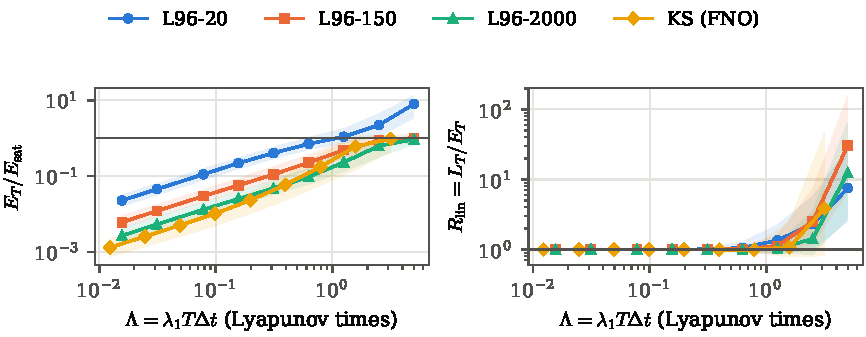
\includegraphics[width=\textwidth]{figures/fig_growth.pdf}
\caption{Error growth. Left: median rollout error relative to the saturation level $E_{\rm sat}$, with 10--90\% bands, as a function of the horizon in Lyapunov times. Right: ratio $R_{\rm lin}$ between the first-order reconstruction and the actual error.}
\label{fig:growth}
\end{figure}

\subsection{Scalar sensitivities}
\label{sec:res_scalar}

Figure~\ref{fig:scalar} shows the within-seed rank correlation between the rollout error and scalar descriptors of the window, as the median over seeds. The worst-case gains $G_{\max}$ and $\|\mathcal L_T\|_2$ and the leading singular value of the one-step Jacobian at the initial state are weak predictors of the error at all horizons. For L96 their correlations lie between $0.09$ and $0.49$, and for KS between $-0.13$ and $0.51$. The total defect magnitude $S_T$ ranks the errors almost perfectly at short horizons and loses most of its value at about one Lyapunov time ($0.49$ for L96 at $\Lambda=1.25$ and $-0.28$ for KS at $\Lambda=0.79$). The norm of the first-order reconstruction keeps a correlation above $0.97$ up to $1.25$ Lyapunov times for L96 and up to $0.79$ Lyapunov times for KS. This is expected, since $\delta^{\rm lin}_T$ is the first-order approximation of $\delta_T$, and it is not an independent explanation of the error. The following sections identify which part of the reconstruction carries the differences between forecasts.

\begin{figure}[t]
\centering
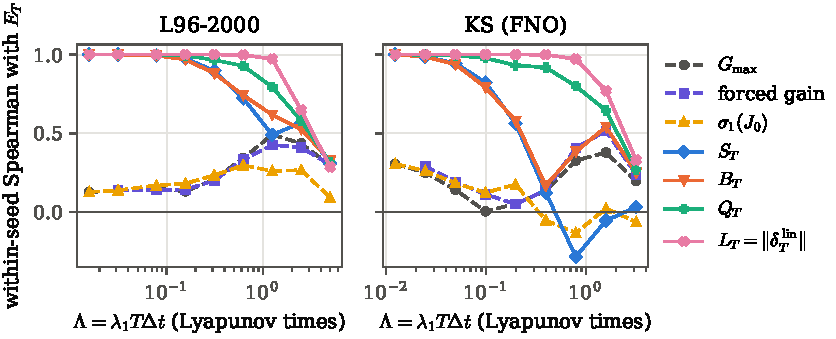
\includegraphics[width=\textwidth]{figures/fig_scalar.pdf}
\caption{Median over seeds of the within-seed Spearman correlation between the rollout error $E_T$ and scalar descriptors of the forecast window. Dashed lines: sensitivity of the learned dynamics only (worst-case initial-value gain, worst-case forced gain and one-step Jacobian). Solid lines: quantities built from the actual defects.}
\label{fig:scalar}
\end{figure}

\subsection{The error budget}
\label{sec:res_budget}

Figure~\ref{fig:budget} shows the five factors of Proposition~\ref{prop:factorization} as geometric means over windows, together with the variance shares of Proposition~\ref{prop:attribution}, and Table~\ref{tab:representative} gives median values at representative horizons. The typical error is built in the same way in both systems. The defect magnitude $S_T$ grows linearly with the horizon and the worst-case tail gain $\bar g_T$ grows approximately exponentially, whereas the efficiency and the cancellation decrease. For L96 at $1.25$ Lyapunov times, the median worst-case estimate $B_T$ exceeds the realized error by a factor of $6.5$, of which a factor of about $3.3$ is removed by the efficiency ($\eta_T=0.31$) and a factor of $1.8$ by the cancellation ($C_T=0.55$). For KS at $0.79$ Lyapunov times, the corresponding values are $4.9$, $\eta_T=0.27$ and $C_T=0.78$, so that the efficiency removes most of the difference.

\begin{figure}[t]
\centering
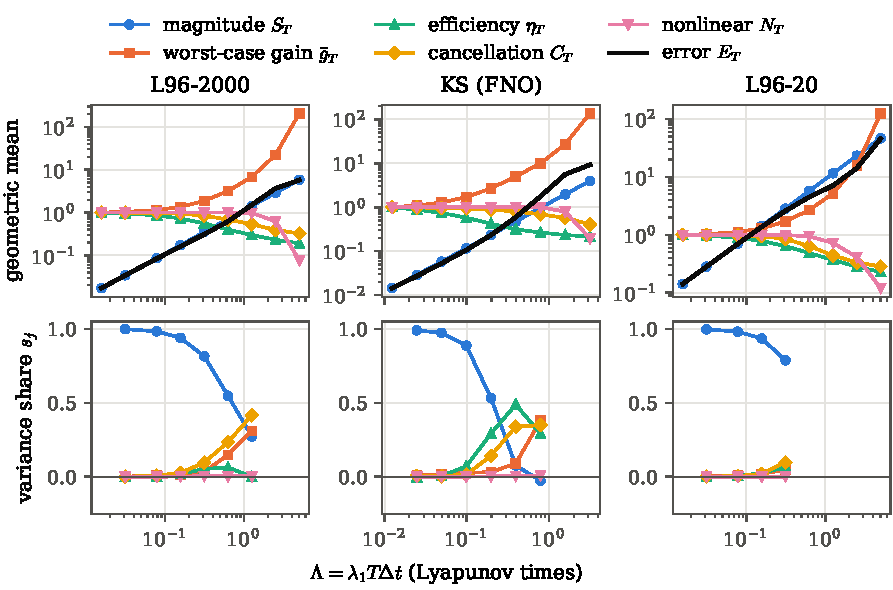
\includegraphics[width=\textwidth]{figures/fig_budget.pdf}
\caption{Error budget. Top: geometric mean over windows of the five factors of Eq.~\eqref{eq:factorization} and of the rollout error. Bottom: variance shares of the log-error (Proposition~\ref{prop:attribution}, within-seed), shown where the median error is below half of the saturation level.}
\label{fig:budget}
\end{figure}

\begin{table}[t]
\centering
\small
\caption{Medians of the budget at representative horizons, and within-seed variance shares of the log-error. $B_T/E_T$ is the ratio between the worst-case first-order estimate and the realized error.}
\label{tab:representative}
\begin{tabular}{lrrrrr}
\toprule
 & L96, $T=40$ & L96, $T=80$ & KS, $T=32$ & KS, $T=64$ & KS, $T=128$\\
\midrule
$\Lambda$ & 0.63 & 1.25 & 0.40 & 0.79 & 1.58\\
$E_T/E_{\rm sat}$ & 0.095 & 0.232 & 0.059 & 0.175 & 0.608\\
$R_{\rm lin}$ & 1.000 & 1.023 & 0.995 & 0.992 & 1.078\\
\midrule
$B_T/E_T$ & 3.6 & 6.5 & 3.6 & 4.9 & 8.1\\
$\bar g_T$ & 3.2 & 6.6 & 4.9 & 9.1 & 23.0\\
$\eta_T$ & 0.40 & 0.31 & 0.32 & 0.27 & 0.24\\
$\eta^\Sigma_T$ & 0.42 & 0.32 & 0.32 & 0.28 & 0.25\\
$\eta^{\rm iso}_T$ & 0.43 & 0.33 & 0.14 & 0.11 & 0.10\\
$\alpha_T$ & 0.96 & 0.94 & 1.03 & 0.97 & 0.96\\
$C_T$ & 0.70 & 0.55 & 0.85 & 0.78 & 0.67\\
$\kappa_T$ & 4.2 & 4.3 & 4.4 & 5.0 & 5.2\\
$\kappa^{\rm iid}_T$ & 1.05 & 1.06 & 1.24 & 1.26 & 1.23\\
$T_{\rm eff}^{1/2}$ & 6.1 & 8.0 & 5.2 & 6.7 & 8.2\\
\midrule
$s_S$ & 0.55 & 0.27 & 0.08 & -0.03 & 0.02\\
$s_{\bar g}$ & 0.15 & 0.31 & 0.09 & 0.38 & 0.61\\
$s_\eta$ & 0.06 & -0.00 & 0.49 & 0.29 & 0.14\\
$s_C$ & 0.24 & 0.41 & 0.34 & 0.35 & 0.39\\
$s_N$ & 0.01 & 0.00 & 0.01 & 0.01 & -0.15\\
\bottomrule
\end{tabular}

\end{table}

The variance shares identify the factors that make some forecasts worse than others. At short horizons, the defect magnitude carries almost all of the variance of the log-error (shares above $0.8$ up to $0.3$ Lyapunov times for L96 and up to $0.1$ Lyapunov times for KS), so that the forecasts that degrade first are those that start in regions of the attractor where the surrogate fits the one-step map less accurately. Geometric factors then replace the magnitude, in a different order in the two systems. For L96, the cancellation and the worst-case gain grow first, and at $1.25$ Lyapunov times their shares ($0.41$ and $0.31$) exceed that of the magnitude ($0.27$, two-level bootstrap interval $[0.20,0.35]$), while the efficiency carries no variance. For KS, the efficiency replaces the magnitude much earlier, with a share of $0.49$ at $0.40$ Lyapunov times, and it is followed by the cancellation and by the worst-case gain, whose share reaches $0.61$ at $1.58$ Lyapunov times. Almost all of the share of the efficiency comes from the orientation ratio $\alpha_T$ ($0.46$, with interval $[0.36,0.65]$, at $0.40$ Lyapunov times), that is, from the variation between windows of the alignment of the defects with the amplified directions. The nonlinear factor carries no variance while the first-order description holds, and its share becomes negative near saturation, where the windows with the largest first-order reconstructions are compressed the most.

The budget changes little with the accuracy of the surrogate. At $0.31$ Lyapunov times, the shares of the magnitude, the cancellation and the worst-case gain differ by at most $0.03$ between the three Lorenz--96 families, and at $0.63$ Lyapunov times they are $0.53$, $0.23$ and $0.13$ for L96-150, against $0.55$, $0.24$ and $0.15$ for L96-2000 (Appendix~\ref{app:tables}). A fiftyfold reduction of the one-step error therefore reduces the error at a given horizon mostly through the magnitude factor, and the dimensionless factors are set mainly by the reference dynamics and by the statistics of the defects.

\subsection{Directional efficiency and the defect covariance}
\label{sec:res_efficiency}

Figure~\ref{fig:efficiency} compares the efficiency of the actual defects with the two null models of Eq.~\eqref{eq:alpha}. For L96, the covariance-matched and isotropic nulls are almost identical, since the defect covariance of the standardized cyclic system is close to isotropic, and the actual efficiency follows both closely. The median orientation ratio is between $0.94$ and $0.99$ up to $1.25$ Lyapunov times. For KS, the isotropic null is much lower than the actual efficiency ($0.11$ against $0.27$ at $0.79$ Lyapunov times), because the defects of the FNO are smooth fields that project mostly on the large scales, which the tail propagators amplify, whereas a random vector of $\R^{64}$ puts most of its energy in strongly damped small scales. Once the spatial structure of the defects is taken into account through $\Sigma$, the actual efficiency is again close to the null, with median orientation ratios between $1.03$ and $1.07$ up to $0.4$ Lyapunov times and of $0.97$ and $0.96$ at $0.79$ and $1.58$ Lyapunov times. For KS, the orientation ratio varies widely between windows (10--90\% range of $[0.56,1.52]$ at $0.79$ Lyapunov times), and this variation carries the share of the efficiency.

\begin{figure}[t]
\centering
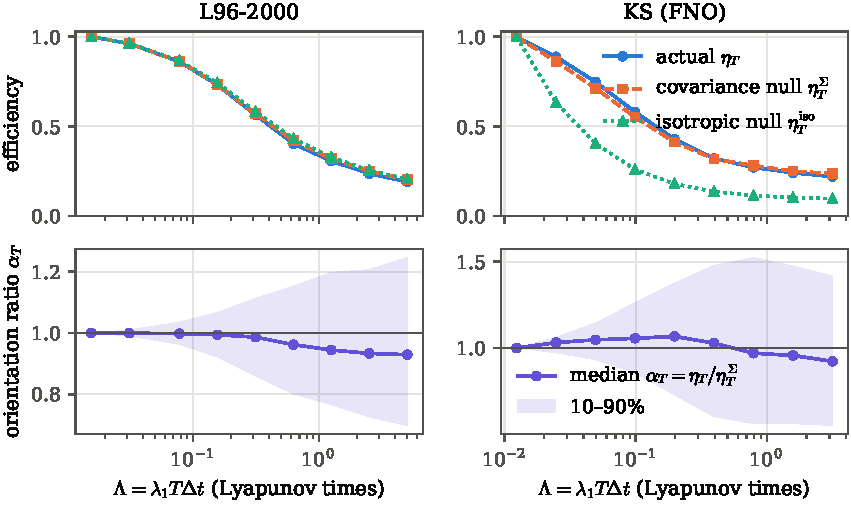
\includegraphics[width=\textwidth]{figures/fig_efficiency.pdf}
\caption{Directional efficiency. Top: median efficiency of the actual defects compared with random defects with the same second moment ($\eta^\Sigma_T$) and with isotropic random defects ($\eta^{\rm iso}_T$), both computed with the mean norm gain of Eq.~\eqref{eq:mean_gain}. Bottom: orientation ratio $\alpha_T=\eta_T/\eta^\Sigma_T$, median and 10--90\% band.}
\label{fig:efficiency}
\end{figure}

The defects of the surrogates are therefore neither attracted to nor repelled by the directions that the dynamics amplify. On average, they realize the fraction of the worst-case gain expected for random draws from their own covariance, within $7\%$ for both systems at all horizons where the first-order description holds. The efficiency decreases with the horizon because, as the singular spectrum of the tail propagators spreads, a vector with a given covariance realizes a decreasing fraction of the leading gain (Proposition~\ref{prop:nulls}). The root-mean-square gains of Proposition~\ref{prop:nulls} would instead have given ratios of $0.89$ at $1.25$ and $0.80$ at five Lyapunov times for L96, close to the Jensen gap $(2/\pi)^{1/2}$, and suggested, incorrectly, that the defects avoid the amplified directions.

The same conclusion holds for the occupation of the singular spectrum (Fig.~\ref{fig:spectrum}). The number of singular directions that carry $90\%$ of the transported energy decreases with the horizon, from $17.6$ at $T=2$ to $3.6$ at five Lyapunov times for L96 (means over defect--tail pairs), and random defects drawn from the defect covariance give $17.5$ and $3.5$. For KS, the actual defects give $6.5$ at $T=2$ and $1.6$ at $3.2$ Lyapunov times, against $7.3$ and $1.6$ for the covariance null, and only the isotropic null departs from them at short horizons ($16.3$ at $T=2$). The concentration of the transported energy in a few leading directions is therefore a property of the propagators and would be observed for any defect.

\begin{figure}[t]
\centering
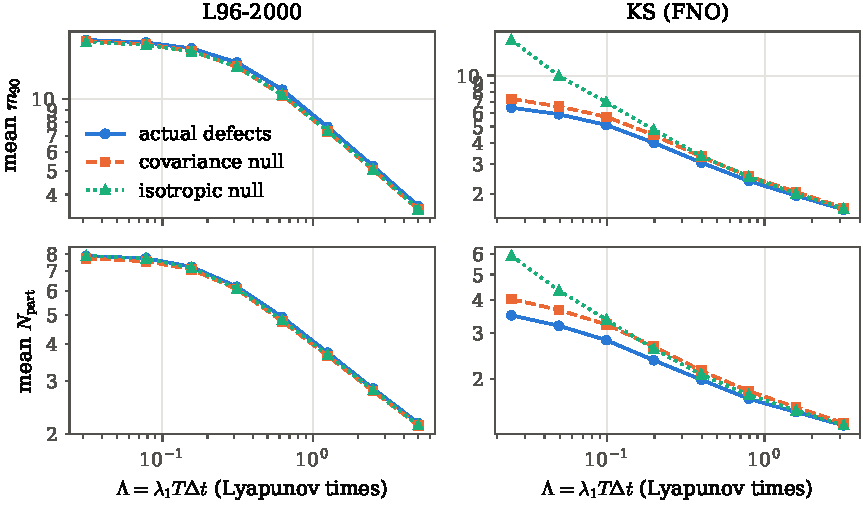
\includegraphics[width=\textwidth]{figures/fig_spectrum.pdf}
\caption{Occupation of the singular spectrum of the tail propagators by the transported defects: number of directions carrying $90\%$ of the energy ($m_{90}$) and participation number, averaged over defect--tail pairs, for the actual defects and for 16 random defects per pair drawn from the covariance-matched and isotropic null models.}
\label{fig:spectrum}
\end{figure}

\subsection{Coherence of the transported defects}
\label{sec:res_coherence}

Figure~\ref{fig:coherence} decomposes the cancellation according to Eq.~\eqref{eq:coherence}. The transported defects are far from incoherent. The coherence factor grows from $\kappa_T=3.8$ at $0.31$ to $4.3$ at $1.25$ Lyapunov times for L96, and from $4.4$ at $0.40$ to $5.2$ at $1.58$ Lyapunov times for KS, against $T_{\rm eff}^{1/2}$ between $4.4$ and $8.2$ for perfectly coherent contributions. The bias of the surrogates explains only a small part of this coherence. Defects drawn independently from a distribution with the same mean and second moment would give $\kappa^{\rm iid}_T$ between $1.04$ and $1.06$ for L96 and about $1.25$ for KS (Eq.~\ref{eq:kappa_iid}), so that the coherence is produced by the temporal correlation of the defects along the trajectory. As the horizon grows, the tail propagators rotate the transported defects into a few leading directions, and the coherence saturates at about four to five while $T_{\rm eff}$ keeps increasing. In the variance attribution, most of the share of the cancellation is carried by $\kappa_T$ (for L96, $0.20$ of $0.24$ at $0.63$ Lyapunov times and $0.32$ of $0.41$ at $1.25$), so that the forecasts with the largest errors are, to a large extent, those whose transported defects add more coherently.

\begin{figure}[t]
\centering
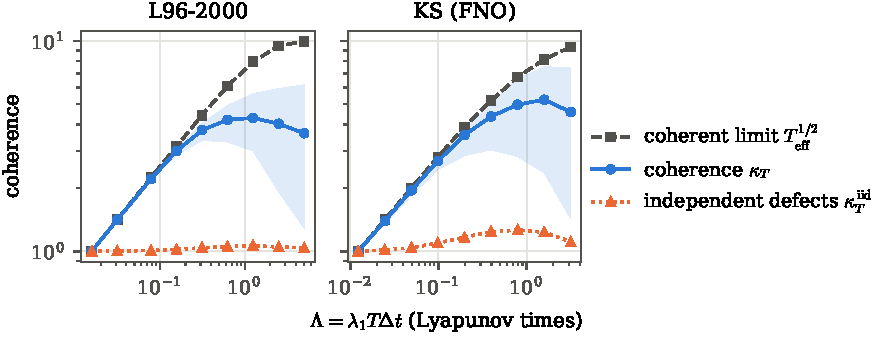
\includegraphics[width=\textwidth]{figures/fig_coherence.pdf}
\caption{Coherence factor $\kappa_T$ of the transported defects (median and 10--90\% band), compared with the coherent limit $T_{\rm eff}^{1/2}$ and with the coherence $\kappa^{\rm iid}_T$ of independent defects with the same mean and second moment (Eq.~\ref{eq:kappa_iid}), which equals one for unbiased defects.}
\label{fig:coherence}
\end{figure}

\subsection{Validity of the first-order reconstruction}
\label{sec:res_validity}

The ratio $R_{\rm lin}$ stays within $2.3\%$ of one up to $1.25$ Lyapunov times for L96, with a median of $1.42$ at $2.5$ Lyapunov times (Fig.~\ref{fig:growth}). For KS, it stays within $1\%$ of one up to $0.79$ Lyapunov times, and its median is $1.08$ at $1.58$ and $3.9$ at $3.2$ Lyapunov times. The departure from the first-order description is controlled by the size of the error relative to the attractor rather than by the horizon (Fig.~\ref{fig:validity}). The median $|\log R_{\rm lin}|$ grows approximately as a power of $E_T/E_{\rm sat}$ and reaches $0.05$ at $E_T/E_{\rm sat}\approx0.20$ for L96, $0.17$ for KS, $0.29$ for L96-150 and $0.54$ for L96-20. The growth is faster for the MLPs (exponents between $2.1$ and $2.5$) than for the FNOs (exponent close to $1.3$). For the accurate surrogates, the first-order reconstruction can therefore be trusted while the rollout error remains below about $15$ to $20\%$ of the saturation level, which corresponds to about one Lyapunov time.

\begin{figure}[t]
\centering
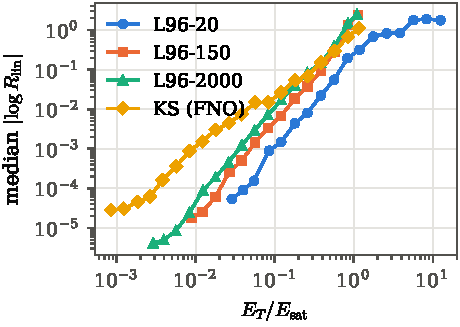
\includegraphics[width=0.6\textwidth]{figures/fig_validity.pdf}
\caption{Median departure from the first-order description, $|\log R_{\rm lin}|$, as a function of the rollout error relative to the saturation level, for windows binned by $E_T/E_{\rm sat}$ and pooled over horizons.}
\label{fig:validity}
\end{figure}

\subsection{Reference-free estimates of the realized error}
\label{sec:res_ensemble}

Since the realized error is determined by the actual defect field and not by its statistics, scores that use only the defect statistics do not rank individual forecasts. For L96, the within-seed rank correlation of $S^{\rm white}_T$ with the error is between $0.08$ and $0.17$ up to $0.31$ Lyapunov times and $0.44$ at $1.25$ Lyapunov times, and the worst-case gain of the model-trajectory propagator behaves in the same way (Fig.~\ref{fig:ensemble}).

The ensemble proxy of Eq.~\eqref{eq:proxy} estimates the defect field itself: on the reference states, its median cosine with the true defect is $0.82$ for the L96-2000 surrogates and $0.84$ for the FNOs, and its median norm is $1.01$ and $1.06$ times the true one, close to the values $0.89$ and $1.12$ expected for independent member errors. This estimate makes the forced recursion usable before the fact (Table~\ref{tab:ensemble} and Fig.~\ref{fig:ensemble}). For L96-2000, the ensemble spread $D_T$ ranks the errors with within-seed correlations between $0.75$ and $0.84$ and flags the 10\% largest errors of each seed with AUROCs between $0.92$ and $0.95$ up to $1.25$ Lyapunov times, and its median ratio to the realized error is between $1.00$ and $1.01$, so that the spread of four other surrogates gives a calibrated estimate of the error of each member. The propagated proxy $\hat L_T$ gives almost the same ranking at the cost of one Jacobian--vector product per step, whereas the proxy magnitude $\hat S_T$ and the one-step proxy fall to $0.50$ and $0.38$ at $1.25$ Lyapunov times. For KS, $D_T$ and $\hat L_T$ keep correlations between $0.67$ and $0.77$ between $0.4$ and $0.8$ Lyapunov times, with AUROCs between $0.92$ and $0.97$, while the magnitude scores become uninformative ($\hat S_T$ has a correlation of $-0.23$ at $0.79$ Lyapunov times). The spread overestimates the KS errors by $7$ to $19\%$ up to $0.79$ Lyapunov times, as expected for nearly independent member errors.

\begin{table}[t]
\centering
\small
\caption{Reference-free scores built from the disagreement of independently trained surrogates (Section~\ref{sec:design_ensemble}). $\rho$: median over seeds of the within-seed Spearman correlation with $E_T$; AUROC for the 10\% largest errors of each seed; $D_T/E_T$: median ratio.}
\label{tab:ensemble}
\begin{tabular}{llrrrrrrr}
\toprule
Surrogate & $T$ & $\Lambda$ & $\rho(\hat e_0)$ & $\rho(\hat S_T)$ & $\rho(\hat L_T)$ & $\rho(D_T)$ & AUROC$(D_T)$ & $D_T/E_T$\\
\midrule
L96-2000 & 10 & 0.16 & 0.72 & 0.83 & 0.83 & 0.84 & 0.93 & 1.01\\
L96-2000 & 40 & 0.63 & 0.51 & 0.68 & 0.79 & 0.78 & 0.93 & 1.01\\
L96-2000 & 80 & 1.25 & 0.38 & 0.50 & 0.74 & 0.75 & 0.92 & 1.00\\
L96-2000 & 160 & 2.50 & 0.30 & 0.58 & 0.61 & 0.63 & 0.80 & 0.90\\
\midrule
L96-20 & 10 & 0.16 & 0.55 & 0.61 & 0.60 & 0.58 & 0.82 & 0.76\\
L96-20 & 40 & 0.63 & 0.43 & 0.72 & 0.69 & 0.70 & 0.84 & 0.81\\
L96-20 & 80 & 1.25 & 0.36 & 0.81 & 0.71 & 0.83 & 0.98 & 0.96\\
L96-20 & 160 & 2.50 & 0.29 & 0.92 & 0.64 & 0.89 & 1.00 & 1.10\\
\midrule
KS & 8 & 0.10 & 0.64 & 0.67 & 0.70 & 0.72 & 0.94 & 1.12\\
KS & 32 & 0.40 & 0.13 & 0.26 & 0.75 & 0.73 & 0.95 & 1.16\\
KS & 64 & 0.79 & 0.07 & -0.23 & 0.77 & 0.67 & 0.97 & 1.19\\
KS & 128 & 1.58 & 0.13 & -0.02 & 0.57 & 0.65 & 0.90 & 0.99\\
\bottomrule
\end{tabular}

\end{table}

\begin{figure}[t]
\centering
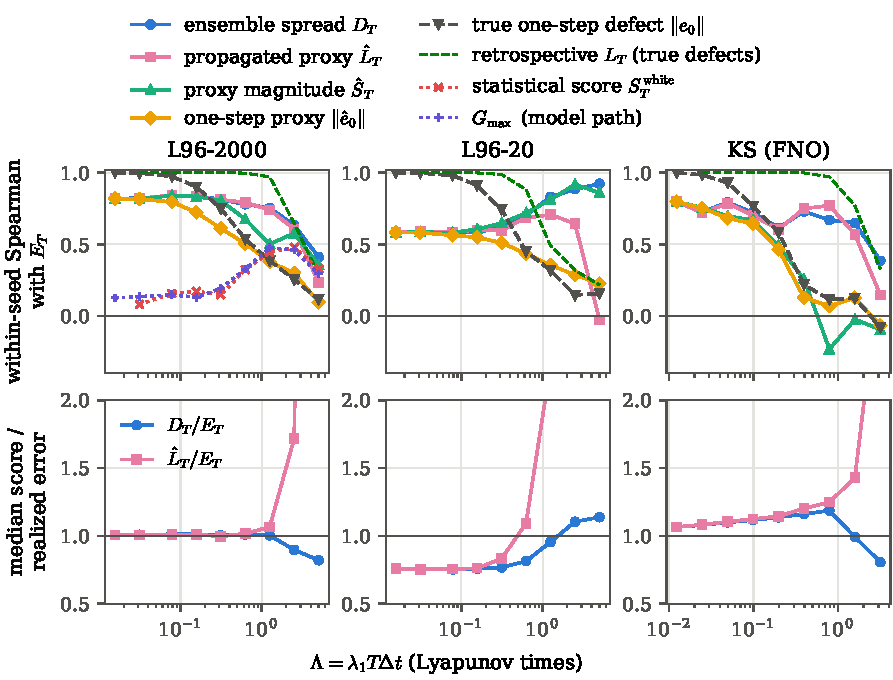
\includegraphics[width=\textwidth]{figures/fig_ensemble.pdf}
\caption{Reference-free error estimates. Top: within-seed Spearman correlation with $E_T$ of the ensemble spread, of the propagated, cumulative and one-step defect proxies, and, for comparison, of the true one-step defect, of the retrospective first-order reconstruction $L_T$ and (L96-2000) of two scores built from the defect statistics only. Bottom: median ratio between the spread or the propagated proxy and the realized error.}
\label{fig:ensemble}
\end{figure}

Two limitations are apparent. First, the under-trained L96-20 surrogates make similar errors, so that the proxy has a cosine of only $0.63$ with the true defect and $77\%$ of its norm, and the spread underestimates the error by $19$ to $25\%$ up to $0.63$ Lyapunov times. Its ranking is nevertheless good at long horizons ($0.83$ at $1.25$ Lyapunov times), where the error of these surrogates is dominated by the drift of their free rollouts. Second, beyond the validity of the first-order description, $\hat L_T$ overestimates the error strongly, whereas the nonlinear spread $D_T$ saturates with the forecasts and remains informative (correlations of $0.63$ for L96 at $2.5$ and of $0.65$ for KS at $1.58$ Lyapunov times).

\subsection{Multistep fine-tuning}
\label{sec:res_intervention}

Figure~\ref{fig:intervention} and Table~\ref{tab:intervention} summarize the fine-tuning study. For the L96-20 surrogates, the rollout arm reduces the test error of all five seeds at every horizon from $T=4$ on, and the median paired reduction grows from $1.2\%$ at $T=16$ to $11.5\%$ at $T=128$ over 312 non-overlapping windows of a common held-out trajectory. The factorization shows how this reduction is obtained. At $1.25$ Lyapunov times ($T=80$), the median over seeds of the mean change of the log-error is $-0.074$, of which $-0.054$ comes from the worst-case tail gain, $-0.010$ from the cancellation and $-0.012$ from the nonlinear factor, whereas the defect magnitude and the efficiency change by less than $0.2\%$. The multistep objective therefore acts on the learned tangent dynamics rather than on the defects. Along the reference trajectory, the median of $\log\sigma_1[\Phir(T,0)]$ of the L96-20 surrogates is already lower than that of the exact tangent map, by $0.26$ at $T=80$; the one-step arm leaves this deficit almost unchanged ($0.28$) and the rollout arm increases it to $0.36$, while the L96-2000 surrogates reproduce the reference value within $0.01$. The rollout arm also reduces the amplitude drift of the free rollout, with a median ratio between forecast and reference amplitudes of $1.19$ at $T=64$, against $1.28$ for the one-step arm. For these under-trained surrogates, the multistep objective thus lowers the error by damping the learned dynamics, at the cost of a larger departure from the reference tangent dynamics.

\begin{figure}[!tp]
\centering
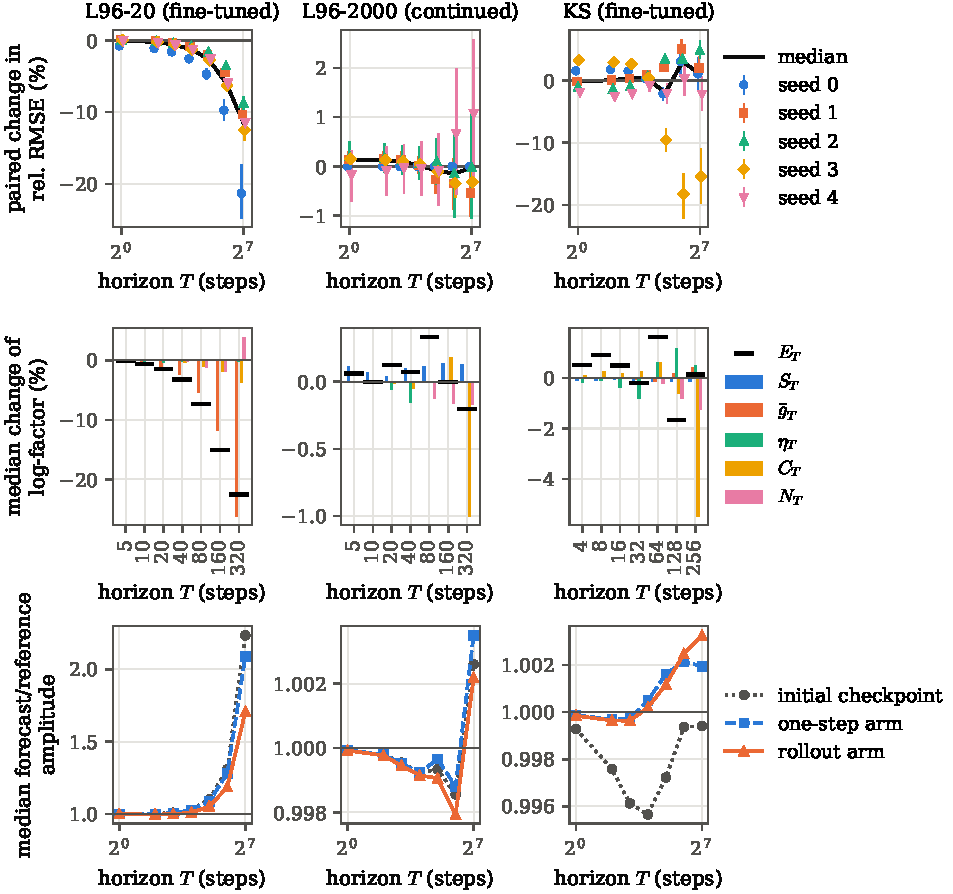
\includegraphics[width=\textwidth]{figures/fig_intervention.pdf}
\caption{Multistep fine-tuning. Top: paired change of the test relative RMSE (rollout arm against one-step arm) for every seed, with window-bootstrap 95\% intervals, and median over seeds. Middle: median over seeds of the mean change of the log-error and of its five factors on the diagnostic windows. Bottom: median ratio between the amplitudes of the forecast and of the reference state.}
\label{fig:intervention}
\end{figure}

\begin{table}[t]
\centering
\small
\caption{Median over five seeds of the paired change of the test relative RMSE (\%) between the rollout and the one-step arms, with the number of seeds improved by the rollout arm. Seed-level values and intervals are given in Appendix~\ref{app:tables}.}
\label{tab:intervention}
\begin{tabular}{lrrrr}
\toprule
Case & $T=16$ & $T=32$ & $T=64$ & $T=128$\\
\midrule
L96-20 & $-1.22$ (5/5) & $-2.60$ (5/5) & $-5.92$ (5/5) & $-11.46$ (5/5)\\
L96-2000 & $+0.02$ (1/5) & $-0.08$ (3/5) & $-0.15$ (3/5) & $-0.03$ (3/5)\\
KS & $+0.44$ (1/5) & $-2.04$ (3/5) & $+3.07$ (1/5) & $+1.09$ (2/5)\\
\bottomrule
\end{tabular}

\end{table}

The converged surrogates do not benefit from the multistep objective. For L96-2000, the paired changes are below $0.2\%$ in median at all horizons, with one to three of five seeds improved, and the window-bootstrap intervals of most seeds include zero. On the diagnostic windows, the mean change of the log-error and of every factor is below $0.4\%$ up to $2.5$ Lyapunov times. For the FNOs, the effects change sign between seeds and horizons. One seed improves by $9.5$ to $18.2\%$ between $T=32$ and $128$, two seeds become worse by $2$ to $5\%$, and the remaining two change sign between horizons (Appendix~\ref{app:tables}). The factors that change also differ between seeds, and neither the magnitude nor the worst-case gain changes systematically. Under the tested budgets, the benefit of the multistep objective in Lorenz--96 is therefore an effect of under-training, obtained by damping a learned map whose free rollouts leave the attractor, and it disappears when the surrogate reproduces the tangent dynamics of the reference system.

\section{Discussion}
\label{sec:discussion}

\paragraph{Available and realized amplification.}
The factorization separates two questions that are often merged. The first is how much amplification the learned dynamics make available, measured by $G_{\max}$, by the forced gain $\|\mathcal L_T\|_2$ or, along a forecast, by $\bar g_T$. The second is how much of it the defects of the surrogate use. In the current experiments, the worst-case estimate $B_T$ exceeds the realized error by a factor of about two at $0.3$ Lyapunov times and by a factor of five to seven at about one Lyapunov time, and the difference is removed by the efficiency and the cancellation in roughly comparable parts. The low efficiency does not indicate that the defects avoid the amplified directions, since random defects with the same second moment realize the same fraction of the available gain, and it decreases with the horizon as the stable rank of the tail propagators (Proposition~\ref{prop:nulls}). The gain that matters for the error of a typical defect is therefore the covariance-weighted gain of generalized stability theory \citep{farrell1996a,farrell1996b} rather than $\sigma_1$, and a bound based on $\sigma_1$, such as the Lipschitz-type bounds commonly used to discuss compounding errors, is pessimistic by a factor that grows with the dimension of the unstable subspace explored by the defects.

\paragraph{Coherence of the defects.}
The transported defects add much more coherently than independent vectors, with coherence factors of four to five at about one Lyapunov time, against $1.05$ to $1.25$ for independent defects with the bias of the surrogates. This is the learned-surrogate counterpart of the quadratic short-time growth of the model error described by \citet{vannitsem2002}, extended to strongly anisotropic tail propagators. Since the coherence comes from the temporal correlation of the defects and not from their mean, removing a constant bias from a surrogate would change little. Objectives that only penalize the size of individual defects, or of individually transported defects, do not act on the cross terms $\mathbf q_j^\top\mathbf q_k$ that make the error grow faster than a random walk, whereas multistep objectives do act on them, since $\|\delta^{\rm lin}_T\|_2^2$ contains all cross terms.

\paragraph{Which factor makes a forecast worse.}
The variance attribution answers a different question from the median budget. Below a few tenths of a Lyapunov time, the defect magnitude explains most of the differences between forecasts. Beyond that, they are explained by the available gain and the coherence and, for the FNO, by the state-to-state variation of the alignment between defects and amplified directions, which is invisible in the median efficiency and appears only in the variance attribution. The worst-case gain, which is the quantity targeted by Jacobian-based regularization \citep{pan2018,nie2026,pervez2026}, becomes the largest single contribution only near and beyond one Lyapunov time, when the first-order description starts to lose accuracy.

\paragraph{Surrogate accuracy.}
Longer training reduces the defect magnitude by about one order of magnitude and extends the first-order regime, but changes the dimensionless factors only moderately. The main qualitative difference is in the nonlinear factor, since the L96-20 surrogates leave the attractor in free run and their errors at about one Lyapunov time already contain an amplitude drift. A surrogate with accurate one-step predictions and accurate Jacobians along the reference trajectory can therefore still have unstable free rollouts \citep{park2024}, and the budget identifies this case through $N_T$.

\paragraph{Multistep fine-tuning.}
The paired attribution shows that the benefit of the multistep objective for the L96-20 surrogates comes from the worst-case gain, that is, from tangent dynamics that become less expansive than those of the reference system, and not from smaller or better oriented defects. Damping the learned dynamics reduces the error of an under-trained surrogate whose free rollouts drift away from the attractor, but it moves the tangent dynamics further from the reference ones, which may degrade other quantities, such as the statistics of long free runs. Surrogates that already reproduce the reference tangent dynamics leave no such margin, and for them the multistep objective changes neither the error nor any factor of the budget. This does not imply that multistep training is ineffective in general, since longer horizons, training from scratch or larger models may behave differently \citep{brandstetter2022,list2025}. It does show that an improvement obtained with a multistep objective should be checked against a converged one-step baseline, and the factorization indicates which part of the budget the objective changed.

\paragraph{Toward prospective use.}
The ensemble estimate of Section~\ref{sec:res_ensemble} turns the retrospective account into a prospective one, and the analysis shows why scores built from the defect statistics fail. The realized error depends on the actual defects along the forecast, through their magnitude in the region of the attractor visited by the forecast, their temporal coherence and their orientation, which no statistic of the defect distribution contains. Independently trained surrogates disagree where they are inaccurate, and their disagreement reproduces these properties well enough to rank the forecasts, provided that the members make sufficiently independent errors, which fails for the under-trained L96-20 surrogates. Ensemble spreads are routinely used as error estimates \citep{leutbecher2008,lakshminarayanan2017}, and the propagated proxy $\hat L_T$ adds a first-order estimate that can be decomposed in the same way as the realized error.

\paragraph{Reference and model propagators.}
Appendix~\ref{app:stress} confirms that the leading right singular vector of $\Phim$ predicts the worst finite-amplitude perturbation of the learned rollout up to sizable amplitudes. This is compatible with the results above: the worst-case direction describes the most dangerous perturbation, but the defects of a surrogate are not drawn from it, and the realized error depends on the full singular spectrum, on the defect covariance and on the coherence of the transported defects.

\section{Limitations}
\label{sec:limitations}

The factorization is exact, but its interpretation in terms of transported defects relies on the first-order reconstruction, whose accuracy is measured in Section~\ref{sec:res_validity}. Beyond that regime, the nonlinear factor $N_T$ absorbs the difference, and the other factors describe the first-order reconstruction rather than the actual error. All quantities are computed in the Euclidean norm of the standardized state. Other metrics (for example, energy norms or task-specific observables) define other singular vectors and other covariance nulls, and could change the efficiencies and the coherence.

The two systems are small enough ($d=20$ and $N=64$) to form every tail propagator explicitly and to compute full singular value decompositions, which costs $\mathcal O(Td^3)$ per window. For high-dimensional surrogates, $S_T$, $L_T$ and $Q_T$ require only Jacobian--vector products, $\sigma_1(\Phi_k)$ can be obtained by power iteration with Jacobian--vector and vector--Jacobian products, and the null models by randomized estimators with a few random vectors or a low-rank $\Sigma$. The full modal accounting of Eq.~\eqref{eq:spectral} would require Krylov approximations of the leading singular subspaces.

The variance shares describe the variability across initial states of a family of surrogates, not a causal decomposition. The surrogates are a residual MLP and a compact one-dimensional FNO trained on single trajectories, and the accuracy of the L96-2000 surrogates is limited by data coverage rather than by optimization (Section~\ref{sec:res_fidelity}). Larger architectures, latent-space models, surrogates trained on many trajectories and surrogates of high-dimensional systems may show different defect structures. The fine-tuning study uses small budgets and a single validation-selected configuration per surrogate family, and its conclusions are restricted to these protocols. In particular, training from scratch with a multistep objective was not tested.

In the fine-tuning study, the 312 evaluation windows are non-overlapping windows of one held-out trajectory and are not necessarily independent, so that the window-bootstrap intervals are conditional on this trajectory and may be too narrow. They do not describe the variability across test trajectories or training protocols.

Finally, the factorization itself is retrospective. The prospective estimate of Section~\ref{sec:res_ensemble} requires several independently trained surrogates, was tested with five members, two systems and moderate dimensions, and does not detect errors shared by all members.

\section{Conclusions}
\label{sec:conclusions}

The long-horizon error of autoregressive surrogates was formulated as a forced finite-time problem and decomposed exactly into the magnitude of the injected defects, the worst-case gain of the tail propagators, the efficiency with which the defects use that gain, the cancellation in the vector sum and a nonlinear remainder. Null models for the efficiency and for the vector composition, together with an exact variance attribution of the log-error, separate the properties of the learned dynamics from those of the learned errors.

For residual MLPs trained on Lorenz--96 with three optimization budgets and for FNOs trained on Kuramoto--Sivashinsky, the worst-case first-order estimate exceeds the realized error by a factor of five to seven at about one Lyapunov time. The defects realize the fraction of the worst-case gain expected for random vectors with their own covariance, but add about four times more coherently than independent ones, because consecutive defects are correlated along the trajectory. The defect magnitude explains which forecasts degrade first, whereas the worst-case gain, the coherence and, for the neural operators, the orientation of the defects explain which forecasts are worse beyond about half a Lyapunov time. These conclusions hold over a sixtyfold range of one-step accuracy, and the first-order description is accurate while the error remains below about 15 to 20\% of the saturation level.

Since the realized error depends on the actual defect field, the disagreement between independently trained surrogates provides a reference-free estimate of it, which ranks individual forecasts up to about one Lyapunov time and, for the converged Lorenz--96 surrogates, predicts the error in magnitude. Multistep fine-tuning reduces the error of under-trained surrogates by damping their tangent dynamics, but it has no consistent effect on surrogates that reproduce the reference tangent dynamics, so that improvements from multistep objectives should be judged against converged one-step baselines. Natural extensions are the use of the factorization with matrix-free estimates for high-dimensional neural operators and weather models, and training objectives that act on the coherence of the transported defects.


\section*{Code and Data Availability}
The source code, the Lorenz--96 surrogates trained with NumPy and the saved results from which all tables and figures are generated are available in the accompanying repository~\citep{fava2026code}. The PyTorch checkpoints of the L96-20 surrogates, of the FNOs and of their fine-tuned versions, together with the results of the campaigns run with them, are distributed as two archives attached to release v1.0.0 of the repository (\url{https://github.com/Thalesclf/jmlr_learned_dynamics_error/releases/tag/v1.0.0}). The repository documentation gives the SHA-256 hashes of the archives and the procedure to restore them.

\appendix
\section{Derivation of the Forced Error Decomposition}
\label{app:derivation}

Let $\mathbf f_k=\mathbf e_k+\mathbf r_k$. Equation~\eqref{eq:error_recursion} gives $\delta_1=\Jr_0\delta_0+\mathbf f_0$ and $\delta_2=\Jr_1\Jr_0\delta_0+\Jr_1\mathbf f_0+\mathbf f_1$. Assume that, for some $T\ge1$,
\begin{equation*}
\delta_{T}=\Phir(T,0)\delta_0+\sum_{k=0}^{T-1}\Phir(T,k+1)\mathbf f_{k}.
\end{equation*}
Multiplying by $\Jr_T$ and adding $\mathbf f_T$ gives the same expression with $T$ replaced by $T+1$, since $\Jr_T\Phir(T,s)=\Phir(T+1,s)$ and $\Phir(T+1,T+1)=I$. Equation~\eqref{eq:error_decomposition} follows by induction, and Eq.~\eqref{eq:linear_error_prediction} is obtained with $\delta_0=0$ and $\mathbf r_k=0$.

\section{Finite-Amplitude Remainder Bound}
\label{app:remainder}

Suppose that $J(\mathbf x)=Df_\theta(\mathbf x)$ satisfies $\|J(\mathbf x)-J(\mathbf y)\|_2\le L_J\|\mathbf x-\mathbf y\|_2$ on a neighborhood containing the segment from $\mathbf x_k$ to $\mathbf x_k+\delta_k$. The integral form of the remainder,
\begin{equation*}
  \mathbf r_k=\int_0^1\left[J(\mathbf x_k+s\delta_k)-J(\mathbf x_k)\right]\delta_k\,ds,
\end{equation*}
gives $\|\mathbf r_k\|_2\le\frac{L_J}{2}\|\delta_k\|_2^2$. Taking norms in Eq.~\eqref{eq:error_decomposition} with $\delta_0=0$,
\begin{equation*}
  E_T\le B_T+\frac{L_J}{2}\sum_{k=0}^{T-1}\sigma_1(\Phi_k)\,\|\delta_k\|_2^2,
\end{equation*}
which is an implicit (discrete Gr\"onwall-type) bound, since $\|\delta_k\|_2$ appears on the right-hand side. The bound is local and becomes uninformative once the error reaches the scale on which $J$ varies, which is the regime identified empirically in Section~\ref{sec:res_validity}.

\section{Proofs of the Propositions}
\label{app:proofs}

\paragraph{Proposition~\ref{prop:factorization}.} The product $S_T\cdot(B_T/S_T)\cdot(Q_T/B_T)\cdot(L_T/Q_T)\cdot(E_T/L_T)$ telescopes to $E_T$. The expressions of $\bar g_T$ and $\eta_T$ as weighted averages follow from the definitions of $w_k$ and $v_k$. Writing $\mathbf e_k=\sum_ic_{ki}\mathbf v_{ki}$ in the right singular basis of $\Phi_k$ gives $\|\Phi_k\mathbf e_k\|_2^2=\sum_i\sigma_{ki}^2c_{ki}^2$, which lies between $\sigma_{k1}^2c_{k1}^2=\sigma_{k1}^2a_k^2\|\mathbf e_k\|_2^2$ and $\sigma_{k1}^2\|\mathbf e_k\|_2^2$, so that $a_k\le\eta_k\le1$. As a weighted average of the $\eta_k$, $\eta_T\in(0,1]$ whenever some transported defect is nonzero. Finally, $0\le L_T\le Q_T$ by the triangle inequality, hence $C_T\in[0,1]$.

\paragraph{Proposition~\ref{prop:nulls}.} For $\mathbf u$ uniform on the unit sphere, $\mathbb E[\mathbf u\mathbf u^\top]=I/d$, so that\[\mathbb E\|\Phi\mathbf u\|_2^2=\operatorname{tr}(\Phi\,\mathbb E[\mathbf u\mathbf u^\top]\,\Phi^\top)=\|\Phi\|_F^2/d=\sum_i\sigma_i^2/d.\] Dividing by $\sigma_1^2$ gives Eq.~\eqref{eq:eta_iso}, and $1\le r(\Phi)\le d$ because $\sigma_1^2\le\sum_i\sigma_i^2\le d\sigma_1^2$. For a random $\mathbf e$ with second moment $\Sigma$, $\mathbb E\|\Phi\mathbf e\|_2^2=\operatorname{tr}(\Phi\Sigma\Phi^\top)$ and, with $\Phi=U\operatorname{diag}(\sigma_i)V^\top$, $\operatorname{tr}(\Phi\Sigma\Phi^\top)=\sum_i\sigma_i^2\mathbf v_i^\top\Sigma\mathbf v_i$. If $\sigma_i/\sigma_1\to0$ for $i\ge2$, then $\sum_i\sigma_i^2/\sigma_1^2\to1$ and $\sum_i(\sigma_i^2/\sigma_1^2)\mathbf v_i^\top\Sigma\mathbf v_i\to\mathbf v_1^\top\Sigma\mathbf v_1$, which gives the two limits. (When $\sigma_2/\sigma_1\to0$, all ratios $\sigma_i/\sigma_1$ with $i\ge2$ also vanish.)

\paragraph{Proposition~\ref{prop:coherence}.} By the triangle inequality and the Cauchy--Schwarz inequality, $L_T\le Q_T\le T_{\rm eff}^{1/2}(\sum_k\|\mathbf q_k\|_2^2)^{1/2}$ with $T_{\rm eff}=Q_T^2/\sum_k\|\mathbf q_k\|_2^2$, which is an identity; the first inequality is an equality if and only if the nonzero $\mathbf q_k$ are positively collinear. This proves (i). Statement (ii) follows from $L_T^2=\sum_k\|\mathbf q_k\|_2^2+2\sum_{j<k}\mathbf q_j^\top\mathbf q_k$. For (iii), $\Phi_k=I$ gives $\delta^{\rm lin}_T=\sum_k\mathbf e_k$; a persistent defect $\mathbf e_k=\mathbf e$ gives $L_T=T\epsilon$, and mutually orthogonal defects of norm $\epsilon$ give $L_T=T^{1/2}\epsilon$.

\paragraph{Proposition~\ref{prop:attribution}.} Since $\log E_T=\sum_j\log X_j$ for every window, the bilinearity of the covariance gives
\[
\operatorname{Var}(\log E_T)=\operatorname{Cov}\Big(\log E_T,\sum_j\log X_j\Big)=\sum_j\operatorname{Cov}(\log E_T,\log X_j).
\]
The identity also holds after every $\log X_j$ is centered within groups of windows (for example, within each trained model), since the centered log-factors still add up to the centered log-error.

\section{Horizon-by-Horizon Diagnostics}
\label{app:tables}

Tables~\ref{tab:h_l96}--\ref{tab:h_ks} list the diagnostics of every surrogate family at every horizon; correlations are medians over seeds of within-seed Spearman correlations with $E_T$ ($\rho_G$ for $G_{\max}$, $\rho_{\mathcal L}$ for the forced gain $\|\mathcal L_T\|_2$, $\rho_S$ for $S_T$ and $\rho_L$ for $L_T$). At $T=1$, the forced gain equals one in every window, and $\rho_{\mathcal L}$ is not defined. The remaining columns are medians over all windows, with $\eta^\Sigma_T$ and $\alpha_T$ computed with the mean norm gains of Eq.~\eqref{eq:mean_gain} and $\kappa^{\rm iid}_T$ from Eq.~\eqref{eq:kappa_iid}. Table~\ref{tab:shares} lists the within-seed variance shares, with the efficiency split into the covariance null and the orientation ratio, $\log\eta_T=\log\eta^\Sigma_T+\log\alpha_T$, and Table~\ref{tab:intervention_seeds} lists the paired effects of the fine-tuning study for every seed.

\begin{table}[h]
\centering\scriptsize
\caption{L96-2000 surrogates.}
\label{tab:h_l96}
\resizebox{\textwidth}{!}{\begin{tabular}{rrrrrrrrrrrrrrr}
\toprule
$T$ & $\Lambda$ & $E_T/E_{\rm sat}$ & $\rho_G$ & $\rho_{\mathcal L}$ & $\rho_S$ & $\rho_L$ & $R_{\rm lin}$ & $\bar g_T$ & $\eta_T$ & $\eta^\Sigma_T$ & $\alpha_T$ & $C_T$ & $\kappa_T$ & $\kappa^{\rm iid}_T$\\
\midrule
1 & 0.02 & 0.003 & 0.13 & -- & 1.00 & 1.000 & 1.000 & 1.00 & 1.000 & 1.000 & 1.000 & 1.000 & 1.00 & 1.00\\
2 & 0.03 & 0.005 & 0.13 & 0.14 & 1.00 & 1.000 & 1.000 & 1.03 & 0.962 & 0.963 & 0.999 & 0.998 & 1.41 & 1.00\\
5 & 0.08 & 0.013 & 0.15 & 0.14 & 0.99 & 1.000 & 1.000 & 1.15 & 0.861 & 0.863 & 0.998 & 0.987 & 2.21 & 1.01\\
10 & 0.16 & 0.025 & 0.13 & 0.14 & 0.98 & 1.000 & 1.000 & 1.36 & 0.732 & 0.735 & 0.994 & 0.950 & 3.00 & 1.02\\
20 & 0.31 & 0.048 & 0.21 & 0.20 & 0.90 & 1.000 & 1.000 & 1.87 & 0.566 & 0.572 & 0.986 & 0.854 & 3.76 & 1.04\\
40 & 0.63 & 0.095 & 0.34 & 0.33 & 0.72 & 0.998 & 1.000 & 3.16 & 0.404 & 0.421 & 0.962 & 0.699 & 4.21 & 1.05\\
80 & 1.25 & 0.232 & 0.49 & 0.43 & 0.49 & 0.971 & 1.023 & 6.56 & 0.307 & 0.321 & 0.945 & 0.554 & 4.30 & 1.06\\
160 & 2.50 & 0.628 & 0.44 & 0.41 & 0.57 & 0.648 & 1.420 & 20.65 & 0.237 & 0.253 & 0.933 & 0.427 & 4.04 & 1.05\\
320 & 5.01 & 0.936 & 0.30 & 0.30 & 0.31 & 0.286 & 12.533 & 183.46 & 0.192 & 0.203 & 0.929 & 0.368 & 3.64 & 1.04\\
\bottomrule
\end{tabular}
}
\end{table}

\begin{table}[h]
\centering\scriptsize
\caption{L96-150 surrogates.}
\label{tab:h_l96_150}
\resizebox{\textwidth}{!}{\begin{tabular}{rrrrrrrrrrrrrrr}
\toprule
$T$ & $\Lambda$ & $E_T/E_{\rm sat}$ & $\rho_G$ & $\rho_{\mathcal L}$ & $\rho_S$ & $\rho_L$ & $R_{\rm lin}$ & $\bar g_T$ & $\eta_T$ & $\eta^\Sigma_T$ & $\alpha_T$ & $C_T$ & $\kappa_T$ & $\kappa^{\rm iid}_T$\\
\midrule
1 & 0.02 & 0.006 & 0.08 & -- & 1.00 & 1.000 & 1.000 & 1.00 & 1.000 & 1.000 & 1.000 & 1.000 & 1.00 & 1.00\\
2 & 0.03 & 0.012 & 0.08 & 0.08 & 1.00 & 1.000 & 1.000 & 1.03 & 0.964 & 0.964 & 1.000 & 0.998 & 1.41 & 1.00\\
5 & 0.08 & 0.030 & 0.07 & 0.07 & 0.99 & 1.000 & 1.000 & 1.14 & 0.867 & 0.868 & 0.999 & 0.987 & 2.21 & 1.01\\
10 & 0.16 & 0.057 & 0.05 & 0.07 & 0.97 & 1.000 & 1.000 & 1.35 & 0.741 & 0.742 & 0.997 & 0.952 & 3.00 & 1.02\\
20 & 0.31 & 0.111 & 0.14 & 0.17 & 0.91 & 0.999 & 1.001 & 1.86 & 0.577 & 0.581 & 0.990 & 0.860 & 3.79 & 1.03\\
40 & 0.63 & 0.228 & 0.28 & 0.30 & 0.73 & 0.989 & 1.009 & 3.13 & 0.422 & 0.434 & 0.985 & 0.701 & 4.26 & 1.05\\
80 & 1.25 & 0.485 & 0.38 & 0.40 & 0.57 & 0.856 & 1.129 & 6.50 & 0.315 & 0.329 & 0.955 & 0.540 & 4.34 & 1.06\\
160 & 2.50 & 0.860 & 0.39 & 0.37 & 0.49 & 0.395 & 2.507 & 21.15 & 0.249 & 0.257 & 0.964 & 0.434 & 4.07 & 1.05\\
320 & 5.01 & 1.021 & 0.12 & 0.12 & 0.17 & 0.091 & 30.502 & 211.35 & 0.205 & 0.207 & 0.973 & 0.396 & 3.81 & 1.04\\
\bottomrule
\end{tabular}
}
\end{table}

\begin{table}[h]
\centering\scriptsize
\caption{L96-20 surrogates.}
\label{tab:h_l96_20}
\resizebox{\textwidth}{!}{\begin{tabular}{rrrrrrrrrrrrrrr}
\toprule
$T$ & $\Lambda$ & $E_T/E_{\rm sat}$ & $\rho_G$ & $\rho_{\mathcal L}$ & $\rho_S$ & $\rho_L$ & $R_{\rm lin}$ & $\bar g_T$ & $\eta_T$ & $\eta^\Sigma_T$ & $\alpha_T$ & $C_T$ & $\kappa_T$ & $\kappa^{\rm iid}_T$\\
\midrule
1 & 0.02 & 0.023 & 0.08 & -- & 1.00 & 1.000 & 1.000 & 1.00 & 1.000 & 1.000 & 1.000 & 1.000 & 1.00 & 1.00\\
2 & 0.03 & 0.045 & 0.09 & 0.10 & 1.00 & 1.000 & 1.000 & 1.03 & 0.971 & 0.971 & 1.001 & 0.999 & 1.41 & 1.01\\
5 & 0.08 & 0.112 & 0.12 & 0.15 & 0.99 & 1.000 & 1.001 & 1.12 & 0.893 & 0.890 & 1.003 & 0.989 & 2.21 & 1.02\\
10 & 0.16 & 0.220 & 0.20 & 0.19 & 0.98 & 0.999 & 1.002 & 1.29 & 0.785 & 0.782 & 1.006 & 0.958 & 3.02 & 1.05\\
20 & 0.31 & 0.407 & 0.24 & 0.26 & 0.92 & 0.988 & 1.006 & 1.69 & 0.642 & 0.635 & 1.010 & 0.857 & 3.79 & 1.08\\
40 & 0.63 & 0.710 & 0.34 & 0.28 & 0.69 & 0.883 & 1.054 & 2.65 & 0.492 & 0.482 & 1.017 & 0.651 & 3.98 & 1.11\\
80 & 1.25 & 1.094 & 0.19 & 0.17 & 0.43 & 0.489 & 1.352 & 5.09 & 0.374 & 0.363 & 1.036 & 0.449 & 3.61 & 1.12\\
160 & 2.50 & 2.225 & 0.08 & 0.08 & 0.24 & 0.319 & 2.306 & 14.77 & 0.289 & 0.277 & 1.030 & 0.351 & 3.38 & 1.10\\
320 & 5.01 & 8.017 & 0.15 & 0.16 & 0.19 & 0.217 & 7.515 & 113.14 & 0.230 & 0.224 & 1.037 & 0.311 & 3.29 & 1.08\\
\bottomrule
\end{tabular}
}
\end{table}

\begin{table}[h]
\centering\scriptsize
\caption{Kuramoto--Sivashinsky FNOs.}
\label{tab:h_ks}
\resizebox{\textwidth}{!}{\begin{tabular}{rrrrrrrrrrrrrrr}
\toprule
$T$ & $\Lambda$ & $E_T/E_{\rm sat}$ & $\rho_G$ & $\rho_{\mathcal L}$ & $\rho_S$ & $\rho_L$ & $R_{\rm lin}$ & $\bar g_T$ & $\eta_T$ & $\eta^\Sigma_T$ & $\alpha_T$ & $C_T$ & $\kappa_T$ & $\kappa^{\rm iid}_T$\\
\midrule
1 & 0.01 & 0.001 & 0.30 & -- & 1.00 & 1.000 & 1.000 & 1.00 & 1.000 & 1.000 & 1.000 & 1.000 & 1.00 & 1.00\\
2 & 0.02 & 0.003 & 0.25 & 0.29 & 0.99 & 1.000 & 1.000 & 1.09 & 0.889 & 0.862 & 1.031 & 0.986 & 1.39 & 1.01\\
4 & 0.05 & 0.005 & 0.14 & 0.19 & 0.94 & 1.000 & 1.000 & 1.27 & 0.748 & 0.713 & 1.047 & 0.976 & 1.95 & 1.04\\
8 & 0.10 & 0.010 & 0.00 & 0.11 & 0.82 & 1.000 & 0.999 & 1.71 & 0.581 & 0.552 & 1.056 & 0.958 & 2.69 & 1.09\\
16 & 0.20 & 0.023 & 0.05 & 0.05 & 0.56 & 1.000 & 0.998 & 2.70 & 0.429 & 0.412 & 1.067 & 0.922 & 3.57 & 1.16\\
32 & 0.40 & 0.059 & 0.13 & 0.14 & 0.12 & 0.999 & 0.995 & 4.90 & 0.322 & 0.319 & 1.028 & 0.851 & 4.37 & 1.24\\
64 & 0.79 & 0.175 & 0.33 & 0.41 & -0.28 & 0.971 & 0.992 & 9.11 & 0.272 & 0.282 & 0.970 & 0.781 & 4.97 & 1.26\\
128 & 1.58 & 0.608 & 0.38 & 0.51 & -0.05 & 0.770 & 1.078 & 23.02 & 0.242 & 0.251 & 0.957 & 0.674 & 5.25 & 1.23\\
256 & 3.16 & 0.964 & 0.20 & 0.24 & 0.03 & 0.329 & 3.860 & 105.46 & 0.221 & 0.237 & 0.922 & 0.498 & 4.59 & 1.11\\
\bottomrule
\end{tabular}
}
\end{table}

\begin{table}[h]
\centering\scriptsize
\caption{Variance shares of the log-error (Proposition~\ref{prop:attribution}) at horizons where the median error is below half of the saturation level.}
\label{tab:shares}
\begin{tabular}{llrrrrrrr}
\toprule
Surrogate & $T$ & $\Lambda$ & $s_S$ & $s_{\bar g}$ & $s_{\eta^\Sigma}$ & $s_\alpha$ & $s_{C}$ & $s_N$\\
\midrule
L96-20 & 2 & 0.03 & 1.00 & 0.00 & -0.00 & 0.00 & 0.00 & 0.00\\
L96-20 & 5 & 0.08 & 0.98 & 0.01 & -0.01 & 0.01 & 0.00 & 0.00\\
L96-20 & 10 & 0.16 & 0.93 & 0.02 & -0.02 & 0.04 & 0.02 & 0.00\\
L96-20 & 20 & 0.31 & 0.79 & 0.05 & -0.03 & 0.10 & 0.10 & 0.00\\
\midrule
L96-150 & 2 & 0.03 & 0.99 & 0.00 & -0.00 & 0.00 & 0.00 & 0.00\\
L96-150 & 5 & 0.08 & 0.97 & 0.00 & -0.00 & 0.02 & 0.01 & 0.00\\
L96-150 & 10 & 0.16 & 0.91 & 0.01 & -0.00 & 0.05 & 0.03 & 0.00\\
L96-150 & 20 & 0.31 & 0.78 & 0.02 & -0.02 & 0.10 & 0.10 & 0.01\\
L96-150 & 40 & 0.63 & 0.53 & 0.13 & -0.07 & 0.16 & 0.23 & 0.01\\
L96-150 & 80 & 1.25 & 0.31 & 0.28 & -0.10 & 0.17 & 0.37 & -0.02\\
\midrule
L96-2000 & 2 & 0.03 & 1.00 & 0.00 & -0.00 & 0.00 & 0.00 & 0.00\\
L96-2000 & 5 & 0.08 & 0.98 & 0.01 & -0.01 & 0.01 & 0.01 & 0.00\\
L96-2000 & 10 & 0.16 & 0.94 & 0.01 & -0.01 & 0.03 & 0.03 & 0.00\\
L96-2000 & 20 & 0.31 & 0.81 & 0.03 & -0.03 & 0.08 & 0.10 & 0.00\\
L96-2000 & 40 & 0.63 & 0.55 & 0.15 & -0.09 & 0.15 & 0.24 & 0.01\\
L96-2000 & 80 & 1.25 & 0.27 & 0.31 & -0.11 & 0.11 & 0.41 & 0.00\\
\midrule
KS & 2 & 0.02 & 0.99 & 0.01 & -0.02 & 0.01 & 0.01 & 0.00\\
KS & 4 & 0.05 & 0.97 & 0.02 & -0.04 & 0.04 & 0.00 & 0.00\\
KS & 8 & 0.10 & 0.89 & 0.03 & -0.06 & 0.13 & 0.01 & 0.00\\
KS & 16 & 0.20 & 0.53 & 0.03 & -0.07 & 0.36 & 0.14 & 0.00\\
KS & 32 & 0.40 & 0.08 & 0.09 & 0.03 & 0.46 & 0.34 & 0.01\\
KS & 64 & 0.79 & -0.03 & 0.38 & 0.00 & 0.29 & 0.35 & 0.01\\
\bottomrule
\end{tabular}

\end{table}

\begin{table}[h]
\centering\scriptsize
\caption{Paired change of the test relative RMSE (\%) between the rollout and the one-step arms for every seed, over 312 non-overlapping windows of a common held-out trajectory, with window-bootstrap 95\% intervals. Negative values indicate a lower error of the rollout arm. For seed 0 of L96-2000, the validation selected the initial checkpoint in both arms.}
\label{tab:intervention_seeds}
\resizebox{\textwidth}{!}{\begin{tabular}{llrrrr}
\toprule
Case & Seed & $T=16$ & $T=32$ & $T=64$ & $T=128$\\
\midrule
L96-20 & 0 & $-2.56$ [-3.15, -2.01] & $-4.71$ [-5.47, -3.89] & $-9.74$ [-11.16, -8.28] & $-21.30$ [-24.78, -17.25]\\
 & 1 & $-0.87$ [-0.95, -0.78] & $-1.94$ [-2.07, -1.80] & $-4.50$ [-4.75, -4.25] & $-10.31$ [-11.25, -9.35]\\
 & 2 & $-0.81$ [-0.91, -0.72] & $-1.62$ [-1.74, -1.50] & $-3.53$ [-3.79, -3.27] & $-8.75$ [-9.72, -7.78]\\
 & 3 & $-1.27$ [-1.40, -1.15] & $-2.75$ [-2.97, -2.55] & $-6.28$ [-6.70, -5.86] & $-12.52$ [-13.94, -11.23]\\
 & 4 & $-1.22$ [-1.32, -1.13] & $-2.60$ [-2.75, -2.46] & $-5.92$ [-6.24, -5.61] & $-11.46$ [-13.11, -9.93]\\
\midrule
L96-2000 & 0 & $+0.00$ [+0.00, +0.00] & $+0.00$ [+0.00, +0.00] & $+0.00$ [+0.00, +0.00] & $+0.00$ [+0.00, +0.00]\\
 & 1 & $+0.02$ [-0.15, +0.19] & $-0.27$ [-0.55, +0.00] & $-0.35$ [-0.87, +0.16] & $-0.54$ [-1.02, -0.06]\\
 & 2 & $+0.06$ [-0.26, +0.40] & $+0.09$ [-0.36, +0.56] & $-0.15$ [-1.03, +0.75] & $-0.03$ [-1.05, +1.10]\\
 & 3 & $+0.04$ [-0.09, +0.17] & $-0.11$ [-0.32, +0.10] & $-0.34$ [-0.62, -0.07] & $-0.32$ [-0.62, -0.00]\\
 & 4 & $-0.04$ [-0.60, +0.51] & $-0.08$ [-0.79, +0.67] & $+0.67$ [-0.57, +1.99] & $+1.08$ [-0.40, +2.58]\\
\midrule
KS & 0 & $+0.39$ [-0.19, +0.99] & $-2.14$ [-3.13, -1.15] & $+3.07$ [+0.61, +5.16] & $+1.09$ [-1.41, +3.79]\\
 & 1 & $+0.93$ [+0.58, +1.27] & $+2.07$ [+1.39, +2.76] & $+5.08$ [+3.46, +6.68] & $+2.04$ [+0.75, +3.82]\\
 & 2 & $+0.72$ [+0.09, +1.39] & $+3.49$ [+2.68, +4.27] & $+3.47$ [+2.22, +4.82] & $+4.84$ [+3.55, +6.42]\\
 & 3 & $+0.44$ [-0.71, +1.61] & $-9.55$ [-11.43, -7.64] & $-18.19$ [-22.13, -14.92] & $-15.38$ [-19.77, -10.98]\\
 & 4 & $-0.81$ [-1.77, +0.05] & $-2.04$ [-3.65, -0.54] & $+0.24$ [-2.42, +3.30] & $-2.19$ [-4.80, +0.61]\\
\bottomrule
\end{tabular}
}
\end{table}

\section{Model-Trajectory Stress Test}
\label{app:stress}

The model-trajectory propagator of Eq.~\eqref{eq:model_propagator} predicts that, for small perturbation amplitudes, the perturbation of the initial state that maximizes the separation of two learned rollouts after $T$ steps is its leading right singular vector $\mathbf v_1^{\rm mdl}$. This prediction is tested with projected gradient ascent (PGD) on
\begin{equation}
  \max_{\|\boldsymbol\epsilon\|_2\le\varepsilon}\ \big\|f_\theta^{(T)}(\mathbf x_0+\boldsymbol\epsilon)-f_\theta^{(T)}(\mathbf x_0)\big\|_2^2,
  \label{eq:pgd}
\end{equation}
with five random restarts, none of which is initialized at $\mathbf v_1^{\rm mdl}$. The nonlinear gain of a unit direction $\mathbf v$ is $G_{\rm NL}(\varepsilon,\mathbf v)=\|f_\theta^{(T)}(\mathbf x_0+\varepsilon\mathbf v)-f_\theta^{(T)}(\mathbf x_0)\|_2^2/\varepsilon^2$. The test uses the L96-2000 surrogates, $T=20$, 20 initial states per seed (100 windows), 200 ascent steps per restart and amplitudes $\varepsilon$ from $10^{-4}$ to $1$. In standardized coordinates, $\varepsilon=1$ corresponds to $20^{-1/2}=22\%$ of the root-mean-square size of the state fluctuations.

At $\varepsilon=10^{-2}$, the mean nonlinear gains of the leading singular direction, of the second singular direction, of a random direction and of the PGD optimum are $9.39$, $6.72$, $1.77$ and $9.40$, and the best of 20 random directions reaches $3.51$. The median alignment $|\mathbf v_1^{{\rm mdl}\top}\mathbf v_{\rm PGD}|$ is $0.999996$, and the median ratio between the two gains is $0.9998$. The median alignment is still $0.9996$ at $\varepsilon=0.1$ and $0.997$ at $\varepsilon=0.3$, and the PGD gain normalized by $\sigma_1^2(\Phim)$ stays within $1.2\%$ of one. At $\varepsilon=1$, the median alignment drops to $0.966$, with a 10\% quantile of $0.82$, and the gain of $\mathbf v_1^{\rm mdl}$ falls to $0.85\,\sigma_1^2$, whereas PGD still finds directions with $0.97\,\sigma_1^2$. The leading singular vector of the model-trajectory propagator therefore describes the most dangerous perturbation of the learned rollout accurately up to about 7\% of the root-mean-square size of the state fluctuations ($\varepsilon=0.3$).

\section{Implementation, Verification and Reproducibility}
\label{app:repro}

The L96-20 surrogates, the FNOs and the fine-tuned FNOs were trained with PyTorch 2.14.0 (CPU) in double precision. All analyses were carried out with an implementation in NumPy and SciPy of the two surrogates, of the two reference integrators with their exact tangent maps, and of all diagnostics, which allows the trained checkpoints to be analyzed without a deep-learning framework. The Jacobians and gradients of the two surrogates and the tangent maps of the RK4 and ETDRK4 steps are written explicitly and checked against finite differences. Applied to the L96-20 checkpoints, the NumPy implementation reproduces the rollout error, the first-order reconstruction, $B_T$, $Q_T$ and $G_{\max}$ of all $4{,}000$ windows of a PyTorch diagnostic campaign with relative differences below $10^{-13}$, and the stored test one-step error of every seed to the last digit. The Lorenz--96 surrogates trained with NumPy use the same data pipeline, a hand-written Adam optimizer and the initialization of \texttt{torch.nn.Linear}. Unit tests check the null models against brute-force Monte Carlo sampling and the exactness of the factorization and of the variance attribution.

The Kuramoto--Sivashinsky reference trajectories are reproducible on a given platform but not bit by bit across platforms, because round-off differences in the FFTs grow at the rate of the leading Lyapunov exponent, and the analyses use new trajectories generated with the initial-condition recipe of the training data. The spatial mean of $u$, an invariant of Eq.~\eqref{eq:ks} fixed by the random initial condition, acts as a Galilean drift, so that all evaluation trajectories are shifted to the mean of the training trajectory ($-2.98\times10^{-3}$). Without this correction, the one-step error of the FNOs on a trajectory with mean $1.4\times10^{-3}$ is about five times larger. The validation trajectory of the Kuramoto--Sivashinsky fine-tuning study had mean $5.7\times10^{-3}$, so that the checkpoint selection used slightly shifted data.


\bibliography{references}

\end{document}
